\chapter{熟悉 \LaTeX}

\LaTeX 是一种基于\TeX 的文档排版系统。\TeX 只这么交错起伏的几个字母,便道出了“排版”二字的几分意味:精确、复杂、注重细节和品味。而\LaTeX 则为了减轻这种写作、排版一肩挑的负担,把大片排版的格式隐藏在若干样式之后,以内容的逻辑结构统帅纷繁的格式,使之成为现在最流行的科技写作——尤其是数学写作的工具之一。

无论你是因为心慕\LaTeX 漂亮的输出结果,还是因为要写论文投稿被逼上梁山,都不得不面对一个事实:\LaTeX 是一种并不简单的计算机语言,不能只点点鼠标就弄好一篇漂亮的文章,也不是一两个小时的泛泛了解就尽能对付得过去。\footnote{不过现代人好像都追求快,沉不下心来。这也是我通过此项目强迫自己学习的理由}

\storybox{\LaTeX 的读音和写法}
{
    \qquad \TeX 一名源自 technology 的希腊词根 $\tau \varepsilon \chi$ ,\TeX 之父高德纳教授近乎固执地要求它的发音必须是(按国际音标) [t$\varepsilon$x],尽管英语中它常被读作[t$\varepsilon$k]。(同样,高德纳教授也近乎固执地要求别人说他的姓 Knuth 时不要丢掉 K ,叫他 Ka-NOOTH ,尽管在英语环境他时常会变成 Nooth 教授。)对比汉语,\TeX 的发音近似于“泰赫”。
    
    \qquad \LaTeX 这个名字则是把\LaTeX 之父 Lamport 博士的姓和\TeX 混合得到的。所以\LaTeX 大约应该读成 “拉泰赫”。不过人们仍然按照自己的理解和拼写发音习惯去读它:
    ['la:t$\varepsilon$k]、['lei:t$\varepsilon$k]或是[la:'t$\varepsilon$k],甚至不怎么合理的['leit$\varepsilon$ks] \footnotemark 。好在 Lamport 并不介意 \LaTeX 到底被读做什么。“读音最好由习惯决定,而不是法令。”—— Lamport 如是说。

    \qquad 两个创始人对于名称和读音的不同态度或许多少说明了这样一个事实:\LaTeX 相对原始的 \TeX 更少关注排版的细节,因此\LaTeX 在很多时候并不充当专业排版软件的角色,而只是一个文档编写工具。而当人们在\LaTeX 中也抱以追求完美的态度并用到一些平时不大使用的命令时,通常总说这是在\TeX 层面排版——尽管\LaTeX 本身正是运行于\TeX 之上的。

    \qquad 类似地,\TeX 和 \LaTeX 字母错位的排版也体现出一种面向排版的专业态度,即使在字符难以错位的场合,也应该按大小写交错写成 TeX 和 LaTeX 。

    \qquad 现在我们使用的\LaTeX 格式版本为$2\varepsilon$ ,意思是超出了第2版,接近却没有达到第3版,因此写成\LaTeXe。在只能使用普通字符的场合,一般写成 LaTeX2e。    
}

\footnotetext{额。我的读法...}

\section{让\LaTeX 跑起来}

学习\LaTeX 的第一步就是上手试一试,让\LaTeX 跑起来。首先安装\TeX 系统及其他一些必要的软件,然后跑一个测试的例子。下面的几节包含了一大堆具体软件安装和使用的内容,虽然比较烦琐,但这是使用\LaTeX 进行写作的必要前提。如果你早已做好这些准备,或者在读本书之前就已经迫不及待地做了不少尝试的话,可以直接跳到开始一个实际的例子。

\subsection{\LaTeX 的发行版及其安装}

\TeX/\LaTeX 并不是单独的程序,现在的\TeX 系统都是复杂的软件包,里面包含各种排版的引擎、编译脚本、格式转换工具、管理界面、配置文件、支持工具、字体及数以千计的宏包和文档。一个\TeX 发行版就是把这样的部件都集合起来,打包发布的软件。

尽管内容复杂,但现在的\TeX 发行版的安装还是非常方便的。下面将介绍两个最为流行的发行版,一是\ref{subsubsec:1} 的 $\mathbb{C}$\TeX 套装,二是\ref{subsubsec:2} 的\texlive 。前者是 Windows 系统下的软件,后者则可以用在各种常用的桌面操作系统上。对 Windows 用户来说,两个发行版并没有显著的优劣之分,你可以任选一个安装使用\footnote{并不是。由于$\mathbb{C}$\TeX 早已停止维护及历史原因,现在\texlive 是更好的选择。于是我选择跳过\ref{subsubsec:1} }。 

\subsubsection{C \TeX 套装}\label{subsubsec:1}

已过时,跳过。

\subsubsection{\texlive} \label{subsubsec:2}

\texlive 是由 TUG ( \TeX User Group ,\TeX 用户组) 发布的一个发行版。\texlive 可以在类 Unix/Linux 、 macOS 和 Windows 系统等不同操作系统下安装使用,并且提供相当可靠的工作环境。\texlive 可以安装到硬盘上运行,也可以经过便携( portable )安装刻录在光盘上直接运行(故有“ Live ”之称)。

不同操作系统下安装设置\texlive 的方式基本一样,这里以 Windows 操作系统为例进行演示。\footnote{原书中还包含部分 Linux 系统上的操作讲解,这里删去。}

\texlive 一般以安装镜像的方式在互联网上发布。光盘镜像文件可以从官网上下载\footnote{\href{https://mirrors.tuna.tsinghua.edu.cn/CTAN/systems/texlive/Images/}{https://mirrors.tuna.tsinghua.edu.cn/CTAN/systems/texlive/Images/}}。载入镜像后,执行 \lstinline{install-tl-windows.bat} 进行安装。只要选好安装的位置,不断单击“下一步”就可以安装\texlive 了,如图所示。

\begin{figure}[H]
    \centering
    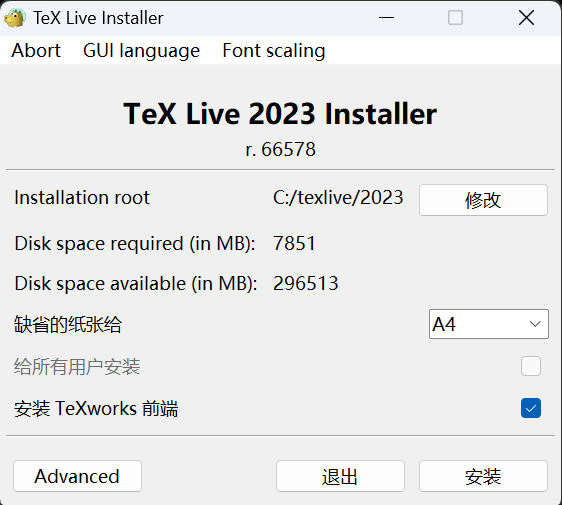
\includegraphics[width=0.6\textwidth]{texlive安装.png}
    \caption{在 Windows 11 上安装 \texlive 2023}
    \label{fig:1}
\end{figure}

程序安装好了之后,会在开始菜单栏增加\texlive 文件夹图标。其中包含的内容比较简单,它包含以下项目:

\begin{itemize}
    \item \textbf{TeXworks editor :} 这是\texlive 预装的一个\TeX 文件编辑器,简单方便。大部分工作都可以在这个编辑器中完成。
    \item \textbf{DVIOUT DVI viewer :} 这是一个 DVI 文件预览器。我们很少用到它。
    \item \textbf{TeX Live command-line :} 它打开 Windows 的命令提示符,并设置好必要的环境变量,可以在其中使用命令行编译处理\TeX 文档。
    \item \textbf{TeX Live documentation :} 这是一个 HTML 页面的链接,里面是\texlive 系统中所有 PDF 或 HTML 格式的文档列表。在首页你可以找到几种语言(包括简体中文)的\texlive 发行版文档,以及到近4000份各种文档的列表的链接——这份有一公里长的列表多少说明了\texlive 是一个多么复杂的系统,以及它在安装时为什么占用了这么大的空间。当然,你不需要读完里面的所有文档才能学会\LaTeX ,不过你会发现在工作中总需要时不时地查看里面的东西。
    \item \textbf{TLShell TeX Live Manager :} 这是\texlive 管理工具的图形界面,简称 \lstinline{tlmgr} 。管理工具也可以在命令行下用 \lstinline{tlmgr} 命令运行,用\lstinline{ tlmgr gui }可以在命令行下打开图形界面。
\end{itemize}

\subsection{编辑器与周边工具}

\subsubsection{编辑器举例——TeXworks}

像其他计算机语言一样,\LaTeX 使用纯文本描述、因而任何能编辑纯文本的编辑器都能编辑\LaTeX 文档,如 Windows 系统的记事本、写字板, Linux 下的 VI 、 GEdit 。不过,使用专门为\LaTeX 设计或配置的编辑器,进行语法高亮、命令补全、信息提示、文档排版等工作,会使工作方便很多。

\LaTeX 代码编辑器有很多,大致可以分为两类:一种主要为\LaTeX/\TeX 代码编辑而专门设计的编辑器,二是可以为\LaTeX/\TeX 代码编辑配置或安装插件的通用代码编辑器。前者如 WinEdt 、 TeXworks 、 TexMaker 、 Kile ,后者如 Emacs 、 VIM 、 Eclipse 、 SciTE 等。 通常前一种编辑器配置和使用更简单一些,下面主要以 TeXworks 为例说明编辑器的一些简单配置。其他大部分编辑器在基本功能和设置上都大同小异,不难举一反三。

TeXworks 的界面非常简洁(见图\ref{fig:2}):它分为两个部分,左侧是\TeX 源文件的编辑窗口,右侧是生成的 PDF 文件的预览窗口。左边的编辑器窗口最上面是标题栏和标准菜单栏,接着是工具栏,中间最大的编辑区,最下面是显示行列号的状态栏。右边的预览窗口把编辑区换成了 PDF 预览区。

\begin{figure}[H]
    \centering
    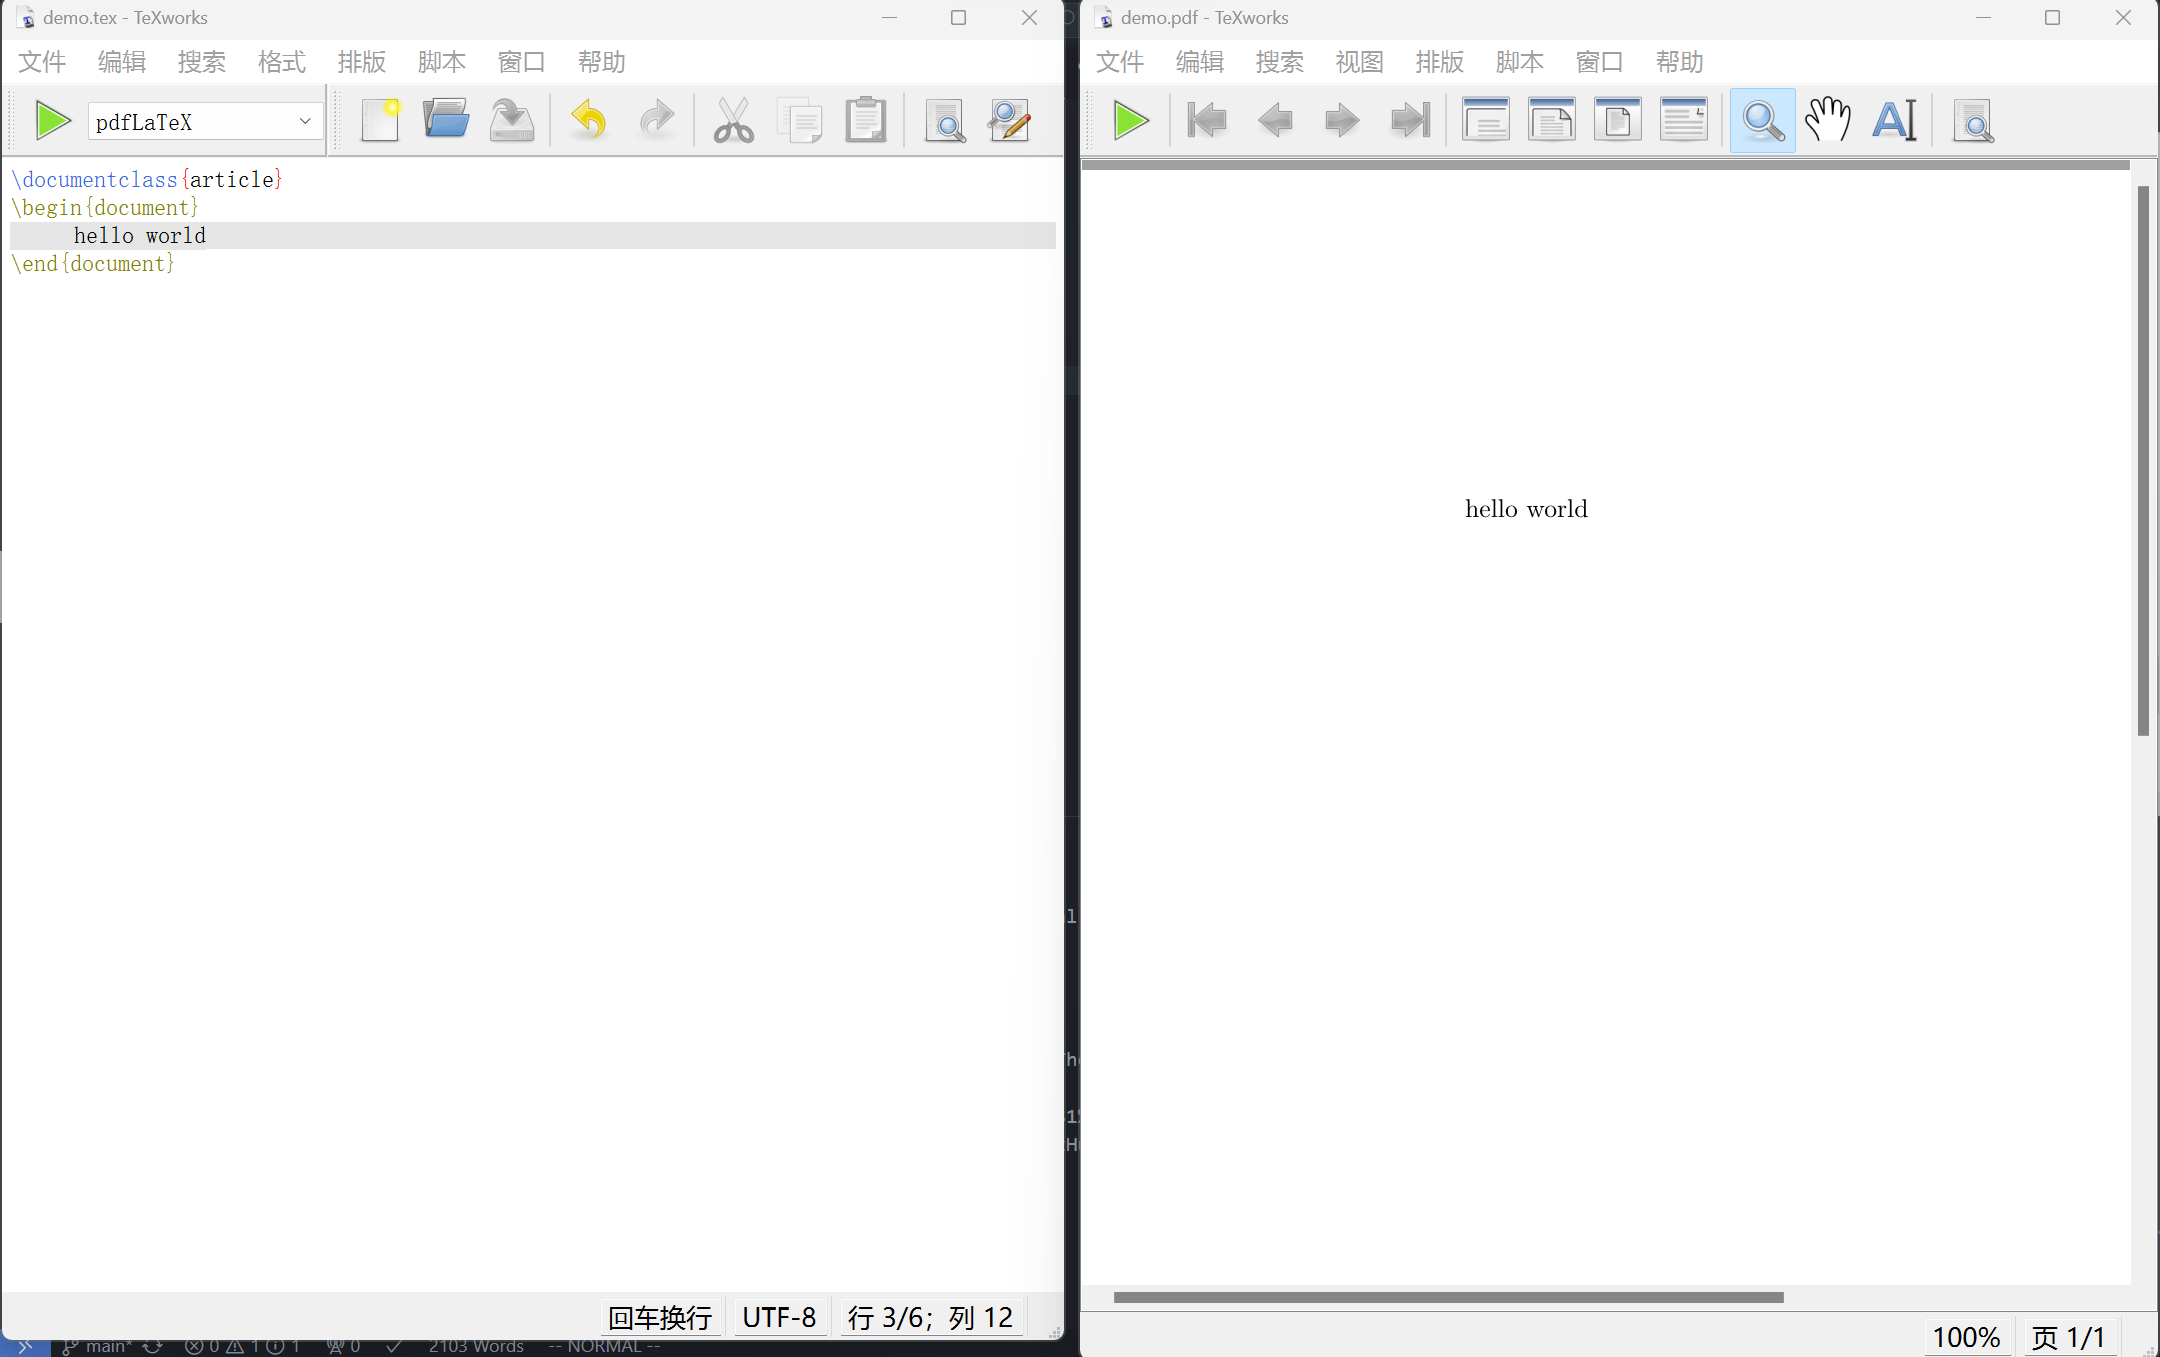
\includegraphics[width=0.6\textwidth]{texworks.png}
    \caption{TeXworks 界面}
    \label{fig:2}
\end{figure}

除了文本编辑区,编辑器窗口中最常用的是工具栏。工具栏的最左边的按钮是整个编辑器最为重要的“排版”按钮,它调用具体的命令把输入的\TeX 源文件\textbf{编译}为对应的 PDF 结果,刷新右边 PDF 文件的显示。紧靠排版按钮右边的下拉菜单中用来选择排版时所使用的命令,通常对应一条单一的命令,但也可以配置为好几条命令的复合。通常我们使用最多的排版命令是“XeLaTeX” 或 “PDFLaTeX”,视具体情况而定。使用排版按钮时,未保存的文档会自动保存。工具栏剩下的按钮则是一系列常见的标准按钮:新建、打开、保存;撤销、重做;剪切、复制、粘贴;查找和替换,不必多说。

PDF 预览窗口的工具栏也是一排按钮。最前面的排版按钮与编辑区的功能一样。右面是4个向前后翻页的按钮;而后是显示比例的按钮;再后面是放大工具、滚屏工具;最后是 PDF 文本查找工具。

使用 TeXworks 也很简单:

\begin{enumerate}
    \item 在编辑区输入 \TeX 源文件
    \item 单击“保存”按钮,给源文件起名并保存在指定位置
    \item 在排版按钮旁的下拉菜单中选择“XeLaTeX”,单击排版按钮,查看结果。
\end{enumerate}

编译时在文本编辑区下方的“控制台输出”面板中会显示编译进度和信息。如果编译过程有错误或提示输入、程序会停下来等待处理。如果编译结束无误,控制台输出面板会自动关闭,而在预览窗口会显示新的 PDF 结果。

在文本编辑区或 PDF 预览区用鼠标左键单击可以从源文件跳转到 PDF 文件中的对应位置;或反过来从 PDF 跳转到源文件中的对应位置。这个功能称为\TeX 文档的\textbf{反向查找},对编写长文档特别有用。正反向查找是由 SyncTeX 机制实现的,需要源代码编辑器、 PDF 阅读器和 \TeX 输出程序的共同参与,一些旧的发行版或程序可能并不支持。

TeXworks 支持\textbf{自动补全}功能。输入一个助记词或命令的一部分,再按 \verb|Tab| 键,则 TeXworks 会根据配置补全整个命令或是环境;连续按 \verb|Tab| 键可以切换补全的不同形式。例如,输入 \verb|\doc| 再按 \verb|Tab| 键,会补全命令 \verb|\documentclass{}|;使用 \verb|beq| 补全则可以得到公式环境:
\begin{lstlisting}
    \begin{equation}
        |
    \end{equation} *
\end{lstlisting}

光标在环境中央等待输入,再次按下 \verb|Ctrl + Tab| 组合键可以跳转到后面的圆点处继续下面内容的输入,而不需要使用方向键。

下面来看看 TeXworks 中一些常见的配置。

刚刚安装的 TeXworks 通常会使用很小的字体,而且可能没有语法高亮等功能,给编辑工作带来诸多不便。在 TeXworks 的“格式”菜单中,“字体”项可以用来临时更改显示的字体,而“语法高亮显示”项可以临时控制如何进行语法高亮。要使字体和语法高亮的设置对所有文档生效,则应该修改 TeXworks 的默认选项。单击 TeXworks “编辑” 菜单的最后一项“首选项”,将弹出 TeXworks 首选项窗口(见图\ref{fig:3})。在“编辑器”选项卡中,可以设置编辑器默认的字体和字号,下面则有语法高亮、自动缩进等格式。

\begin{figure}[H]
    \centering
    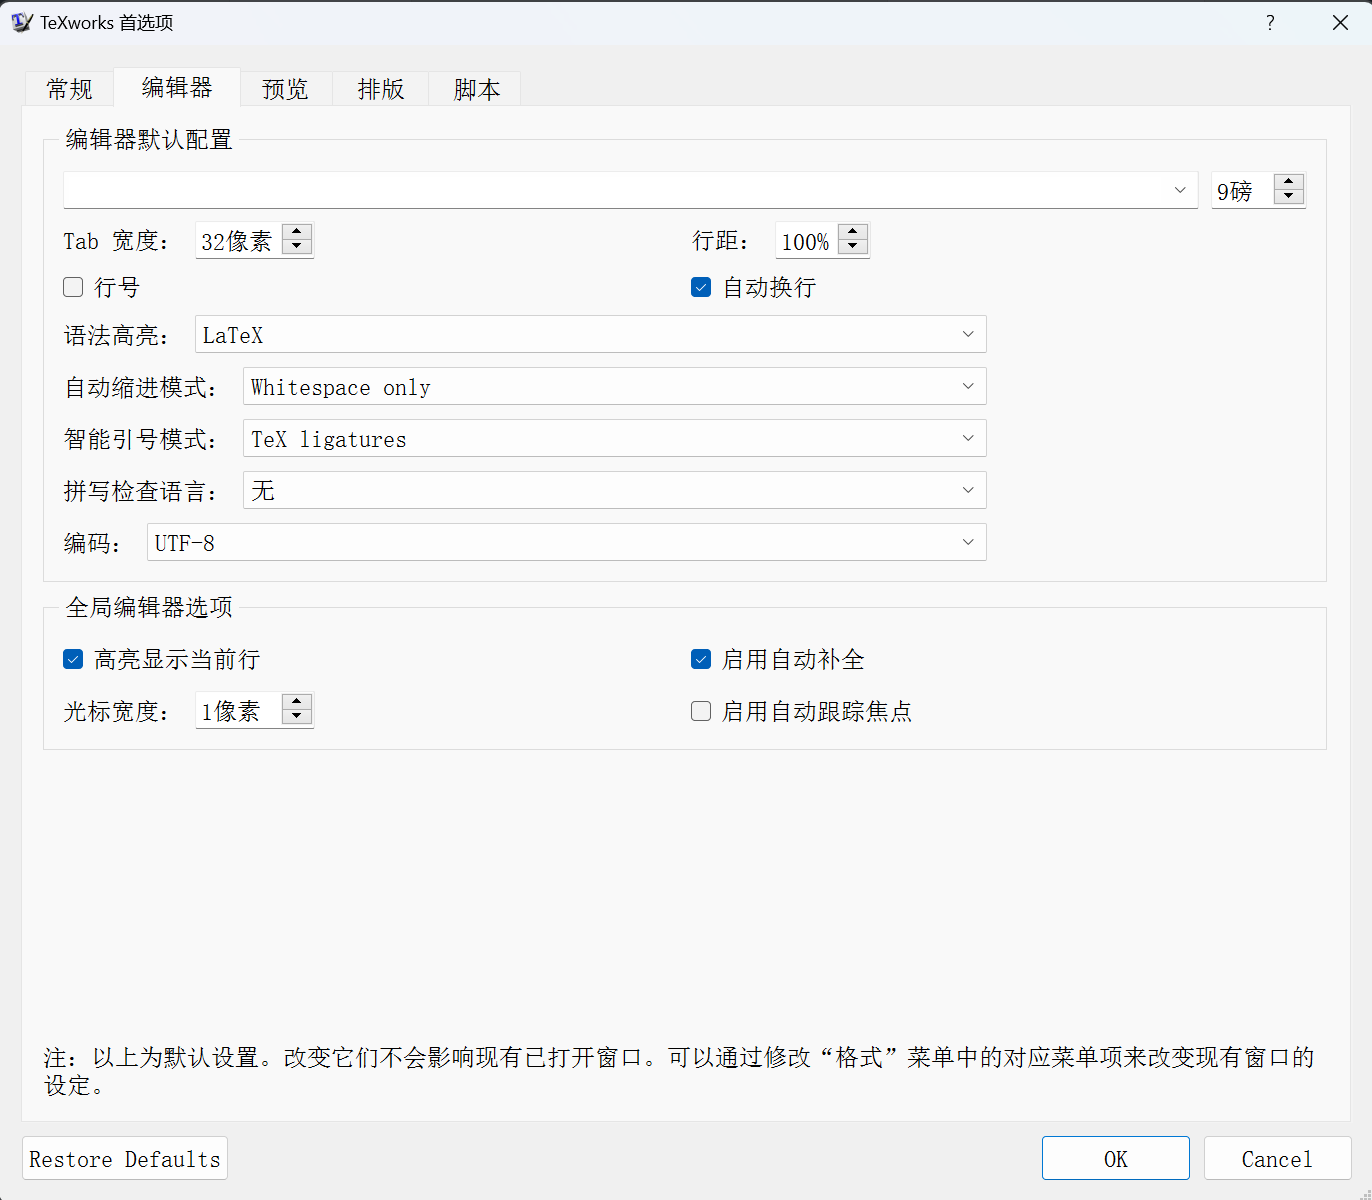
\includegraphics[width=0.4\textwidth]{首选项.png}
    \caption{TeXworks 编辑器首选项设置}
    \label{fig:3}
\end{figure}

TeXworks 支持多种语言界面和多种文字编码。 TeXworks 默认的界面会与操作系统的默认语言( Locale 设置)一致,可以在首选项设置窗口的“一般”( General )选项卡中设置程序的界面语言为中文。在“编辑器”选项卡中则有“编码”选项,一般应选择 TeXworks 的默认值,即 UTF-8 编码,编辑器保存和打开文件将默认使用此编码。

TeXworks 首选项窗口的“排版”选项卡可以用来设置 TeXworks 的“排版”按钮所执行的命令。选择对应的处理工具,单击“编辑...”按钮,就可以在弹出的窗口中设置对应的命令及参数。参数中使用的变量,可参见 TeXworks 的帮助文档。

\begin{figure}[H]
    \centering
    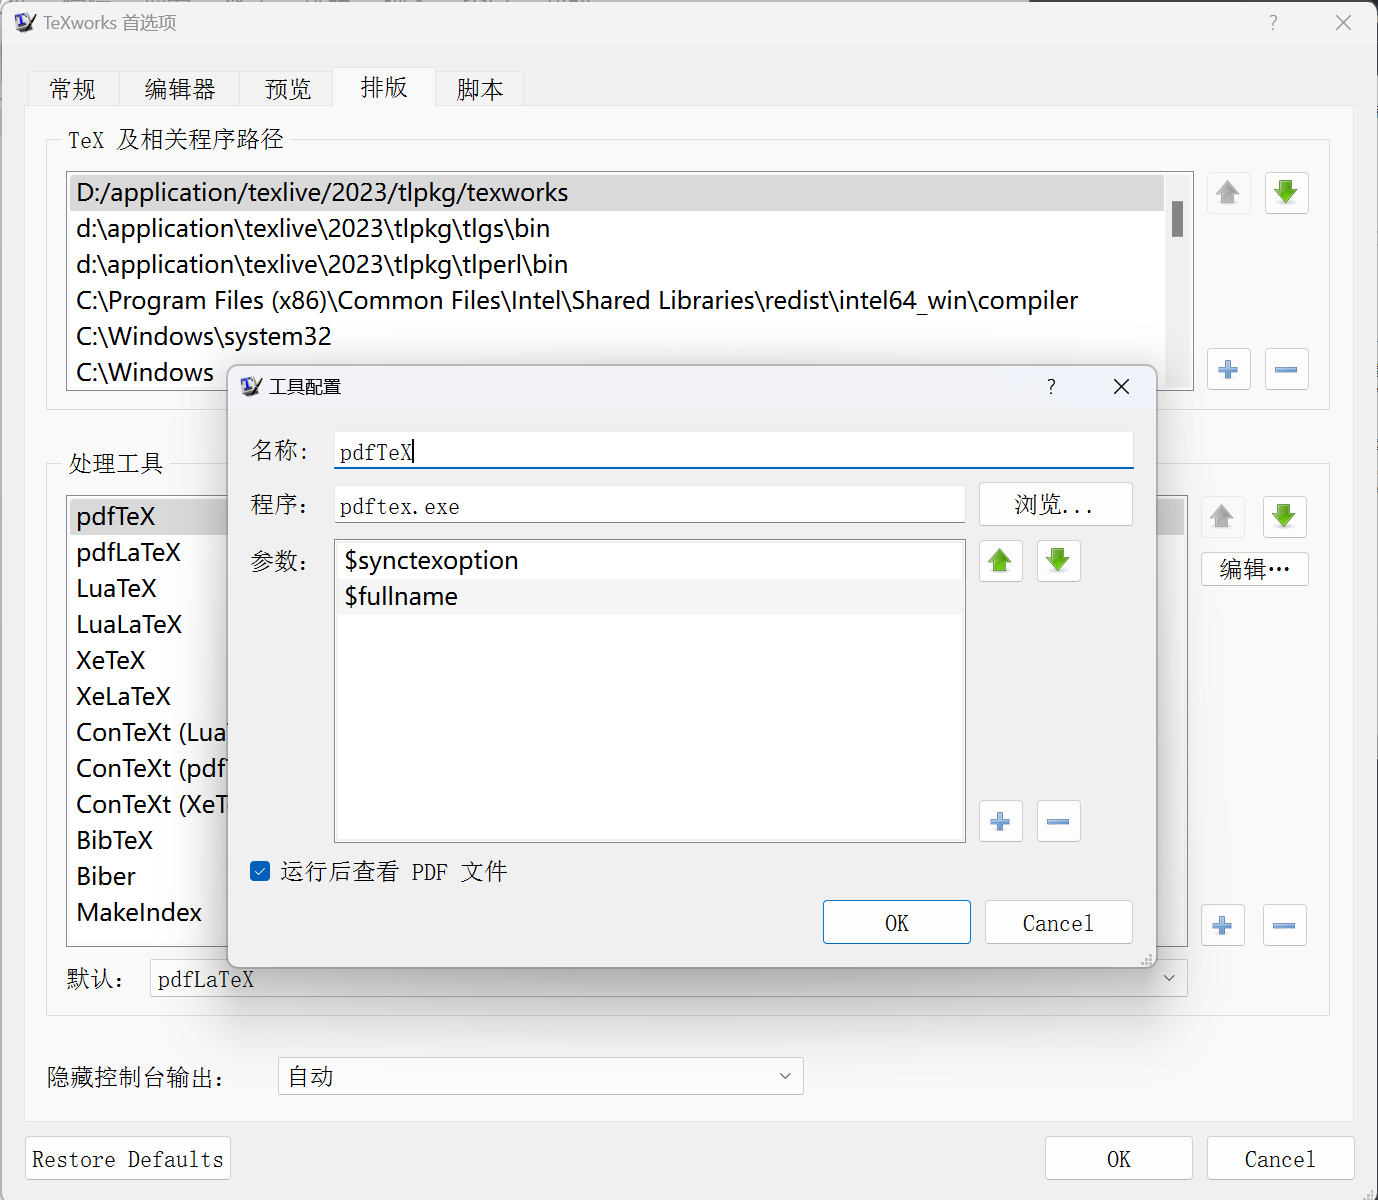
\includegraphics[width=0.5\textwidth]{排版首选项.png}
    \caption{TeXworks 排版首选项设置}
    \label{fig:4}
\end{figure}

\storybox{文本编码与 Unicode}
{
    \qquad 在使用\TeX 编辑器时,必须要注意文档保存的文字编码。如果编码使用错误,轻则遇到“乱码”,重则导致程序运行错误。我们提到的“UTF-8”编码,就是现在最为常用的编码之一。

    \qquad 文字在计算机内部都是以数字的形式表示、储存和运输的,人们圈定一些在计算机中使用的字符,称为字符集( character set ),一个字符通常就用它在字符集中的序号来表示。不过由于在计算机中数字的二进制表示也有不同的格式,因而相同的字符集也可能有不同的二进制表示方式,也就是字符编码( character encoding )。 IBM 公司以前给自己系统中每一种编码编一个号,即所谓代码页( code page ),后来其他计算机厂商如微软、 Oracle 都把自己的字符编码用代码页的方式给出,不过使用的代码页编号都不一样。我们通常见到的代码页,都是微软公司的编号。字符集、字符编码、代码页这些概念,在很多时候都不加区分,可以混用。

    \qquad ISO 于 1990 年推出了通用字符集 ( Universal Character Set, UCS )标准 ISO 10646 , 包括 UCS-2 和 UCS-4 两种长度的编码;1991 年一个叫做通用码协会 ( Unicode Consortium ) 的组织发布了 Unicode 1.0 标准。两个组织都打算把全世界所有文字的符号都用一套字符集和编码统一起来。后来,两个组织协作起来,从 Unicode 2.0 起, Unicode 就符合 ISO 10646 了。 2012年1月发布的 Unicode 6.1 已经定义了 110181 个字符,包括世界上100种文字,而且还在不断修订拓充之中。\footnotemark Unicode 已逐渐成为字符编码的新方向, 包括 GB 18030 也可以看成是 Unicode 字符集的一种编码格式。除了 UCS-2 和 UCS-4 , Unicode 标准还提出了多种编码形式,称为 Unicode 交换格式 ( Unicode Transformation Format, UTF ):主要包括变长的 UTF-8 、 UTF-16 和定长的 UTF-32 编码。 UTF-8 编码与 ASCII 编码向下兼容,因而最为常用。

    \qquad \TeX 系统原本只支持 ASCII 编码。但只要设置好超过127的数字对应的符号,所有拓展 ASCII 编码都能正确排版, 如 ISO 8859 的各种标准。汉字编码 GB 2312 、 GBK 和 UTF-8 都是兼容 ASCII 的多字节编码,因而在 \LaTeX 中通过 CJK 宏包 也可以通过特殊的方式,把多个字符对应到一个汉字上,支持中文的排版。

    \qquad CJK 宏包这种支持多字节编码的方法其实是一种黑客手段,后来 \TeX 的新实现 XeTeX 和 LuaTeX 都直接支持 UTF-8 编码,新的中文排版方式也自2007年起随着这两种新排版引擎应运而生。LuaLaTeX 的本地化支持目前还暂处于起步阶段,本书将着重介绍基于 XeTeX 的方式。
    }

\footnotetext{目前最新版本的 Unicode 13.0 中,包含的字符总数已达143859个。}

\subsubsection{PDF 阅读器}

\texlive 已经预装了 DVI 文件和 PostScript 文件的阅读器。然而却没有安装最重要的 PDF 格式阅读器。现在使用的 \TeX 系统基本上最终都输出 PDF 格式的结果,而且 \TeX 系统中的大部分文档也都是 PDF 格式的,因此一个 PDF 阅读器是不可或缺的。

PostScript 阅读器 GSview 和 PS\_View 也都可以当做 PDF 阅读器来使用,不过效果不是很好。我们使用 PDF 阅读器有两个目的,一是在编辑文档过程中随时查看编译的效果,这对于编辑复杂公式、插图以及幻灯片来说都非常重要;二是为了阅读 PDF 格式的文档资料,或查看自己编写文档的最后效果。这两个目的各有不同的要求,前者要求快捷方便,最好还能在 PDF 的效果和 \TeX 源文件之间方便地切换检索;后者则要求显示准确美观、功能全面。

要满足第一个要求,编辑器 TeXworks 内置的显示功能最为方便。 TeXworks 把源代码和 PDF 结果左右排开,对照显示, \TeX 代码编译后右边的 PDF 文件就会更新。而且可以用 \verb|Ctrl|加鼠标左键单击进行从源文件到 PDF 文件或 PDF 文件到源文件的正反向索引。

要满足第二个要求,我们建议使用 Adobe Reader 最新的版本\footnote{全名为 Adobe Acrobat Reader }( Linux 系统中通常称为 arcoread )。 Adobe Reader 是官方免费提供的 PDF 格式阅读器,通常它的显示结果最好,支持全面的 PDF 特性(如 JavaScript 脚本、动画、3D 对象等,而且这些很可能在 \LaTeX 制作的幻灯片中使用到。)其他一些常见的 PDF 阅读器,如 Foxit Reader ,则可能在一些功能上有欠缺。

如果你还没有安装 Adobe Reader ,可以直接从 Adobe 的官方,或几乎任何的下载站点中得到并安装。不必抱怨它占用上百兆的安装空间:除了一些高级功能的插件, Adobe Reader 还提供了许多种高质量的 OpenType 西文字体,这些都可以在你未来的排版中用到。

\storybox{PS 格式和 PDF 格式}
{
    \qquad PS 是 PostScript 的简称。 PostScript 是 Adobe 公司于1984年发布的一种页面描述语言,自1985年苹果公司的 LaserWriter 打印机开始,此后的很多高档激光打印机都带有 PostScript 。 于是, PostScript 逐渐成为电子与桌面出版的标准格式,并一直延伸到整个出版业,风靡一时。就连国内最大的北大方正公司的排版系统也是以变形的 PostScript 格式输出,并沿用至今。

    \qquad “PostScript”这个名字多少体现了这门语言的特点:它是一种基于后缀表达式和栈操作的解释型计算机语言。例如,表达式 1+2 就被写成 \lstinline{ 1 2 add } 。 而 \lstinline{ 0 0 moveto ; 100 100 lineto } 则是在描述从坐标(0,0)到坐标(100,100)的直线路径。使用这种后缀语法原本是为了方便计算机芯片高效解释 PostScript 这种复杂的语言, 大部分 PostScript 代码也都是由其他计算机程序自动生成的。不过,富有经验的老手可以就凭借着这种看起来有些怪异的语法直接画出图来,这种技艺也一直延伸到将要讲到的 \lstinline{ PSTricks }宏包中。

    \qquad PostScript 拥有强大的图形能力,可以用一段 PostScript 语言的代码表示很复杂的图形。然而,作为一门完整的计算机语言, PostScript 过于复杂,因而出现了所谓封装的 PostScript ( Encapsulated PostScript ) 格式,即 EPS 格式。 EPS 格式的文件也是一段 PostScript 代码,但只能表示一页,而且加上了诸多限制,成为一种专门用来存储可以嵌入其他应用的图形格式。\TeX 的许多输出引擎都支持这种图形格式。

    \qquad 由于在电子出版领域的地位, PostScript 一度成为 \TeX 最重要的输出格式,至今也能在网络上见到大量 \TeX 系统产生的 PostScript 格式的书籍和文章,一些期刊也一直要求以能生成 PostScript 格式的 \TeX 文档投稿。然而随着新一代廉价的喷墨打印机的出现,需要复杂解释芯片的 PostScript 打印机逐渐式微;而网络技术的发展进一步催生了电子文档交换的需求, PDF —— Portable Document Format (可移植文档格式)便应运而生。 PDF 由 Adobe 公司于 1993 年发布,它是 Adobe Acrobat 系列产品的原生文件格式,并随着文件格式的公开和阅读器 Adobe Reader 免费的发放,迅速风靡起来。

    PDF 和 PostScript 使用相同的 Adobe 图形模型,可以得到与 PostScript 相同的输出效果,而在程序语言方面则比 PostScript 大为削减,并增强文档格式结构化,可以迅速地由计算机处理。尽管 PDF 最初只是 PostScript 削减功能 适应电子文档处理的结果,但 PDF 转而在电子文档交互式表单、多媒体嵌入等方面大下功夫,并不断进行各方面的扩充,最终成为一种比 PostScript 还复杂的格式。 PDF 也继 PostScript 之后成为现在新一代的电子出版业的事实标准。

    \qquad 现代的 \TeX 输出引擎几乎都以 PDF 为输出格式。同时 PDF 格式 也可以像 EPS 格式一样作为图形格式被 \TeX 和其他软件使用。现在能够输出 PDF 图形的软件和支持嵌入 PDF 图形的 \TeX 引擎比 EPS 格式的还要多些, PDF 也成为现在 \TeX 系统中最重要的图形格式。

}

\subsubsection{命令行工具}

\textbf{一、命令行}

尽管大多数常用编译操作可以在编辑器中完成,\texlive 还给出了图形界面的配置工具,但 \TeX 发行版的主体仍然是命令行下的程序。不了解命令行,就难以了解 \TeX 的处理流程,也不能很好地使用诸如 Makeindex 这样的基本 \LaTeX 工具。因此,有必要对命令行和一些命令行工具的使用做一个了解。

命令行是以文字形式与计算机交互的方式,与图形方式相对。在 Windows 系统中,命令行通常由命令行解释程序 \verb|cmd.exe| 处理;在 Linux 及其他类 UNIX 操作系统中,命令行解释程序通常称为 Shell ,最常见的 Shell 是 Bash 。 在命令行下可以执行一些基本的文件操作,也可以运行其他程序,批处理脚本也是由命令行解释程序执行的。 Linux 中 shell 的使用一般远比在 Windows 中频繁,因此这里仍以 Windows 为例。

Windows 中默认的命令行解释程序 \verb|cmd.exe| 可以在“开始”菜单搜索框中输入 \verb|cmd| 查找到 “命令提示符” 进入。如果使用频繁,可以在桌面或任务栏中创建快捷方式,或设定快捷键随时使用。

使用 \TeX 经常需要在特定文件所在的目录进行命令行操作,这时只需要在资源管理器的地址栏内输入 \verb|cmd| 回车。

打开命令行窗口之后,会显示命令提示符,默认的命令提示符由当前盘符、目录和一个大于号 \verb|>| 组成,如
\begin{lstlisting}
    C:\>
\end{lstlisting}
表示当前目录是 C 盘的根目录 \verb|>| 。后面的光标等待输入命令, Windows 命令行命令和文件名不区分大小写,输入一行命令按下回车键即开始执行。

使用最频繁的命令是文件列表命令 \verb|dir| ( directory 的缩写 ),直接输入 \verb|dir| 后按下回车就会显示当前目录下所有文件的详细列表。 \verb|dir| 命令后可以指定要列出的盘符、目录和文件名,如
\begin{lstlisting}
    dir C:\WINDOWS
\end{lstlisting}
将列出 C 盘 WINDOWS 目录下的所有文件。

目录和文件名可以使用 \verb|?| 和 \verb|*| 作为通配符。 \verb|?| 可以替代任意一个字符, \verb|*| 可以代替任意多个字符。例如,命令
\begin{lstlisting}
    dir book*.tex
\end{lstlisting}
将列出所有以 \verb|book| 开头,后缀为 \verb|.tex| 的文件。目录和文件名可以用 \verb|Tab| 键自动补全,如输入 \verb|book| 后,连按 \verb|Tab| 将交替地补全当前目录所有以 \verb|book| 开头的文件。有两个特殊的目录名 \verb|.| 和 \verb|..| 分别用来表示当前目录(可省略不写)和当前目录的上一级目录。

\verb|cd| 命令 (或 \verb|chdir| , change directory 的缩写)用来改变当前所在的目录。如
\begin{lstlisting}
    cd pictures
\end{lstlisting}
将进入当前目录下的 \verb|pictures| 目录(如果有的话),而从 C 盘用命令
\begin{lstlisting}
    cd \WINDOWS\Fonts
\end{lstlisting}
则进入 Windows 的字体目录。注意更换盘符不能用 \verb|cd| 命令,而要单独使用盘符后加冒号 \verb|:| 进入,如输入
\begin{lstlisting}
    D:
    cd \test
\end{lstlisting}
将进入 D 盘根目录下的 \verb|test| 目录。

把多个命令行写到一个文件中,保存为后缀为 \verb|.bat| 或 \verb|.cmd| 的文件,就得到一个批处理文件(又称为批处理脚本)。在命令行下可以像运行其他程序一样调用批处理文件,也可以在图形界面鼠标点击批处理文件执行。批处理可以一次完成多项任务,如完成多道工序的 \TeX 源文件编译工作。批处理还提供命令行参数、变量定义、文件判断等简单的编程功能,详细内容可参见微软的联机帮助。

\textbf{GhostScript}

GhostScript 是一种 PostScript 的解释器,它的主体也是命令行工具。 Windows 版本的 \texlive 附带安装了一份简化版本的 GhostScript , 程序名为 \verb|rungs| 。 一般还是最好单独下载安装完全版本的 GhostScript\footnote{\href{https://www.ghostscript.com/releases/gsdnld.html}{https://www.ghostscript.com/releases/gsdnld.html}} , 因为一些 \LaTeX 输出引擎有时仍会调用它。

可以用 GhostScript 查看 PostScript 或 PDF 格式的文件, PostScript 文件查看器 GSview 和 PS\_View 都是调用 GhostScript 工作的。 GhostScript 更常用的功能是进行文档格式转换,做 PS 、 PDF 格式的相互转换,或把它们转换为点阵图片格式,如 PDF 输出引擎 DVIPDFMx 就会在处理 ERS 图片时自动调用 GhostScript 。

GhostScript 为一些常用的转换提供简单的命令,最常见的是从 \verb|.ps| 到 \verb|.pdf| 文件的转换,可以用 \verb|ps2pdf| 命令完成,如
\begin{lstlisting}
    ps2pdf foo.ps
\end{lstlisting}
命令会将 \verb|foo.ps| 文件转换为 \verb|foo.pdf| 。类似的命令还包括 \verb|pdf2ps| 和 \verb|ps2eps|等。

所有显示和转换的工作都可以通过 GhostScript 的主程序完成。 GhostScript 的主程序是一个命令行程序,在 Windows 下名叫 \verb|gswin64.exe|,在 Linux 等系统下通常叫做 \verb|gs| , 也可以使用 \texlive 的 \verb|rungs| ,这里统一用 \verb|GS| 表示。一个调用 \verb|GS| 的命令通常带有许多命令行参数,以完成各种复杂的操作,例如,
\begin{lstlisting}
    GS -dBATCH foo.ps
\end{lstlisting}
将使 GhostScript 在屏幕上显示 \verb|foo.eps| 的内容并退出;下面的命令(第一行末的\verb||| 并不存在,只表示延续到下一行):
\begin{lstlisting}
    GS -q -sDEVICE=png256 -dEPSCrop -r128 -dGraphicsAlphaBits=4 \
        -dTextAlphaBits=4 -o bar.png foo.eps
\end{lstlisting}
则把 \verb|foo.eps| 转换为 256色 PNG 图像 \verb|bar.png| ,使用128dpi 的分辨率,裁剪到适当大小,并对文字和图像做边缘抗锯齿处理。关于 GhostScript 的详细命令行参数可以参考 GhostScript 的联机文档。

\textbf{三、 ImageMagick}

ImageMagick 是一款优秀的基于命令行的位图处理软件,可以在超过100种不同的图像格式之间转换,或对图像进行各种变换和处理。熟悉平面设计的人可以把它看做是 Adobe Photoshop 这类软件的一些图像滤镜的命令行版本。 ImageMagick 并不直接与 \TeX 相关,但 \TeX 用户经常用它来做一些有关图形转换的工作,个别与 \TeX 相关的软件(如 Asymptote )也会调用 ImageMagick 。

ImageMagick 是自由软件,可以在 \href{https://imagemagick.org/script/download.php}{https://imagemagick.org/script/download.php}进行下载安装。

在 Windows 下安装 ImageMagick 可以在开始菜单栏中找到它的帮助文档和 ImageMagick 中唯一的图形界面程序 IMDisplay 。 但注意 IMDisplay 只是一个图片查看器,并不具备任何 ImageMagick 的图像处理功能,我们主要还是在命令行下使用 ImageMagick 。

ImageMagick 是个很复杂的软件,包括 10多个不同的命令行工具,具有 200多种不同的命令行参数。这里只介绍 ImageMagick 最基本的图像类型转换功能,也是最常用的功能,更详细的功能可以参见 ImageMagick 的联机帮助文档。

命令 \verb| convert | 用于图像的转换,即把一幅图像转换为另一幅图像,尽管功能复杂,但基本的使用方法是十分简明的,如:
\begin{lstlisting}
    convert foo.bmp bar.png
\end{lstlisting}
是将 BMP 格式的图像  \verb| foo.bmp | 转换为 PNG 格式的图像 \verb| bar.png | ,类似地,
\begin{lstlisting}
    convert foo.eps bar.jpg
\end{lstlisting}
则是把 EPS 格式的图片 \verb| foo.eps | 转换为 JPG 格式的图片 \verb| bar.jpg |  。不过 ImageMagick 在处理涉及 PostScript 和 PDF 格式的图片时,内部实际还是调用 GhostScript 来完成的,这时可以把它看做是 GhostScript 命令的一种方便的变形。

\storybox{获取命令行帮助}
{
    \qquad 熟练的用户使用命令行完成一些工作比使用图形界面的软件更高效快捷。不过对于刚接触命令行不久的人来说,命令行的最大问题就是记不住命令的用法,因此应该了解如何在命令行下获取帮助信息。

    \qquad 专门的联机文档或在线文档是比较通用的帮助形式,如在 Windows 下,由 “开始”菜单栏进入联机帮助,以“命令行”、“cmd”等关键字搜索,很容易就能得到详尽的命令行帮助。有时帮助文档则以专门的文件储存,如 GhostScript 和 ImageMagick 在 Windows 下都提供网页形式的帮助文档,可以在“开始”菜单栏中找到。也有很多程序提供 CHM 、 PDF 格式的文档。

    \qquad 另一种方式是直接在命令行下得到帮助,这通常是通过特殊的命令行参数得到的。通常, Windows 命令行的基本命令后加 \lstinline{\/?} 参数获得帮助。如输入 \lstinline{dir \/?}可以在屏幕上获取到 \lstinline{dir} 命令的帮助信息。来自类 UNIX 系统的程序命令行选项以 \lstinline{-}开头,命令行帮助通常可以在命令后加上 \lstinline{--help} 获得。如输入\lstinline{ convert --help } 将会在屏幕上得到关于 ImageMagick 的所有命令行选项的说明。

    \qquad 类 UNIX 系统在命令行下还有一个 \lstinline{man} 命令,可以用来调出文档。如用 \lstinline{ man ls } 将在命令行中直接调出 \lstinline{ ls }命令 (相当于 Windows 系统下的 \lstinline{dir} 命令)的详细帮助,类似的文档程序还有 \lstinline{info} 。在 Windows 中,用 \lstinline{ help } 可以达到类似的效果,不过效果与使用  \lstinline{\/?}  选项差不多。 \TeX 系统继承了 UNIX 中 \lstinline{man} 的用法,也提供了一个 \lstinline{texdoc} 程序,可以在命令行下 调出 \TeX 宏包、工具和字体等的文档。
}

\subsection{“ Happy \TeX ing 与 “特可爱排版”}

在做完所有的准备工作后,我们一起来运行一个简单的例子,测试整个系统。

首先,打开你的 \TeX 编辑器,如 TeXworks ,新建一个文件,输入下面的内容:
\begin{lstlisting}[numbers=left]
    \documentclass{article}

    \begin{document}
    This is my first document.

    Happy \TeX ing !
    \end{document}
\end{lstlisting}

新建一个测试用的目录,将刚刚输入的文件保存到这个目录里面,选择 PDFLaTeX 或者 XeLaTeX 命令,点击编辑器上对应的排版按钮。如果一切顺利,将在 PDF 预览窗口看到编译的结果,内容类似下面的样子:

\begin{figure}[H]
    \centering
    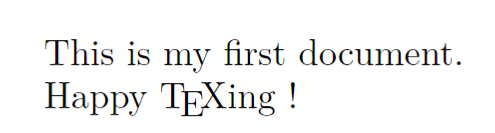
\includegraphics[width=0.3\textwidth]{第一段代码.png}
\end{figure}

这个文件中有一些以反斜杠\verb|\| 开头的语句,大多没有出现在最终的 PDF 文档中。虽然我们之前没有接触过这些语句,不过不难猜测其涵义:\verb|\documentclass{article}| 声明了文档的类型是一篇文章;\verb|\begin{document}| 和 \verb|\end{document}| 语句标识出正文的范围;至于正文中的 \TeX ,看结果就知道它表示“\TeX” 这个高低不平的符号。这是我们的第一个例子,看起来很简单。

可是,如果你马上兴致勃勃地把里面的内容换成汉字,再点击按钮看结果时,就会发现汉字并没有出现在 PDF 中,只有英文字符出现,这是因为 \TeX 原本是面向西文写作的,默认并没有加载中文字体。

通过更换文档类型,下面这个稍稍复杂的例子可以正确显示出中文:
\begin{lstlisting}[numbers=left]
    \documentclass[UTF8]{ctexart}

    \begin{document}
    \section{汉字}
    特可爱排版
    \section{数学}
    \[
        a^2 + b^2 = c^2
    \]
    \end{document}
\end{lstlisting}


\begin{figure}[H]
    \centering
    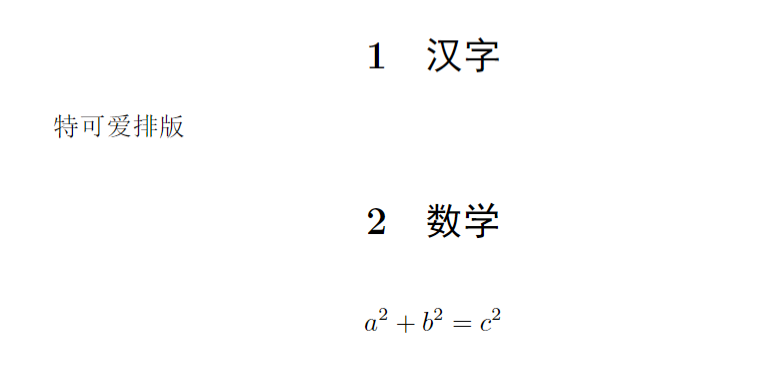
\includegraphics[width=0.5\textwidth]{第一段ctex代码.png}
\end{figure}

这段代码其实也不难看懂:文档类换成了 \verb|ctexart|, 即中文 \TeX 的文章( article )类型,这个文档类使得中文可以正确地显示;在\verb|ctexart| 前面的 \verb|UTF8| 是使用这个文档类的选项,表明了中文所使用的编码;两个 \verb|\section| 命令各自生成了一节的标题;唯一不大直观的是由 \verb|\[| 和 \verb|\]| 包裹起来的数学公式,不过 \LaTeX 数学公式的能力太出名了,你一定早就听说过它了。

上面两个简单的例子给了我们一个 \LaTeX 的直观印象,而且正确运行它们也许能够增强你学习 \LaTeX 的信心。粗略地看,\LaTeX 是一种标记式排版语言,有相关背景的人大概会觉得\LaTeX 的代码与 HTML 代码有很多相似之处,整个文档通过一些标记(命令)分成结构化的部分。\LaTeX 的命令以反斜线 \verb|\| 开头,命令一般以英文单词命名,有的可以带参数。通过一个程序的处理,我们称为 \textbf{编译} 过程, \LaTeX 源代码就能生成对应的输出结果,通常就是一个 PDF 文档。

\begin{figure}[H]
    \centering
    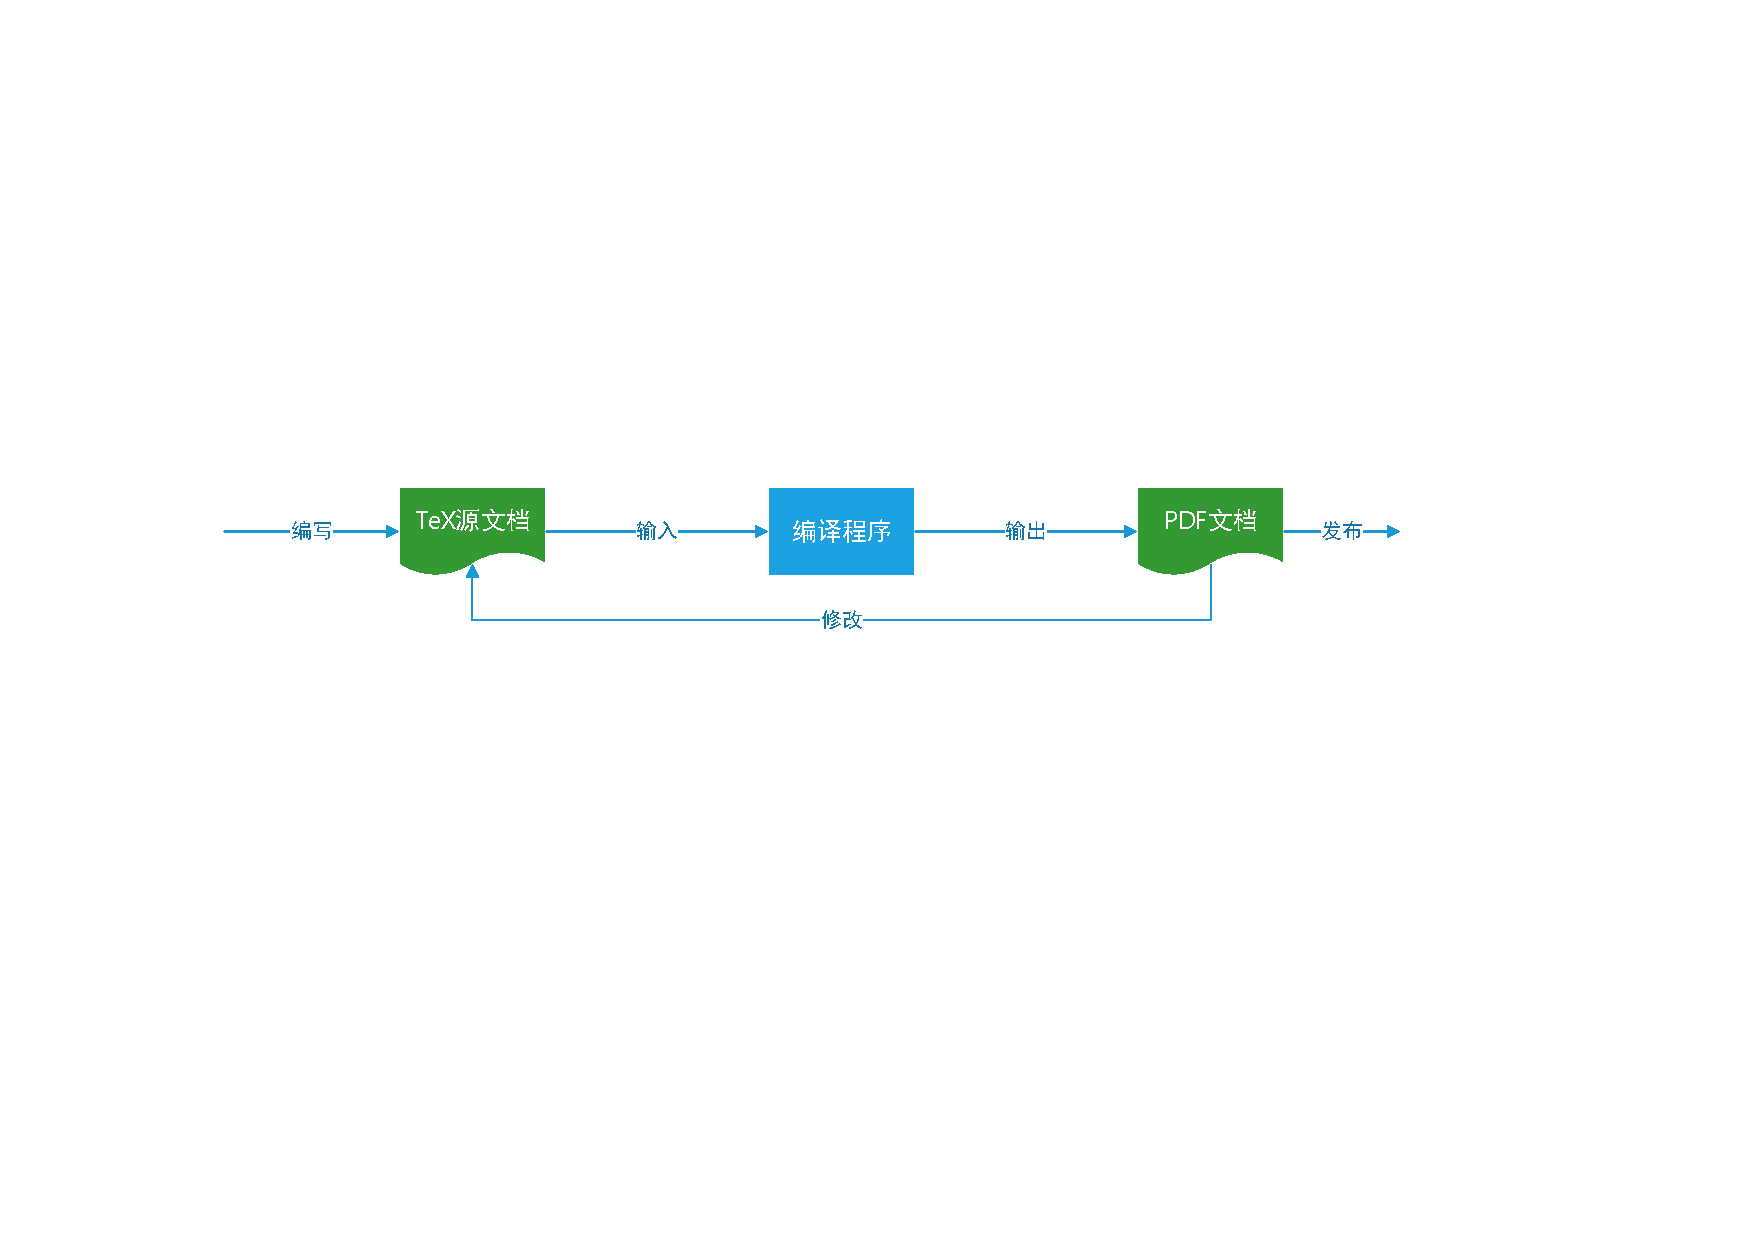
\includegraphics[width=\textwidth]{latex写作流程.pdf}
    \caption{\LaTeX 文档的写作流程}
    \label{fig:5}
\end{figure}

\LaTeX 的写作流程见图\ref{fig:5}。通常这个流程都是自动化完成的,编写 \TeX 源文件通常是在专门的 \TeX 编辑器中进行,例如 TeXworks ,而后按下一个按钮,源文件就会被送给 \TeX 的编译程序进行处理,输出 PDF 文件,此时编辑器调用 PDF 阅读器查看结果。如果出了问题,需要根据输出的结果或程序的错误信息修改源文件或编译方式。

\storybox{编译程序}
{
    \qquad TeXworks 等编辑器里面给出了许多编译程序的按钮,往往让人有种应接不暇的感觉,如果你留心来自各种书籍、文档和网络的资料,上面介绍的编译方法五花八门。如果是使用命令行编译,则输入起来更觉头疼,那么,这些不同的编译程序做了什么?该如何选择和使用呢?

    \qquad 高纳德设计的 \TeX 原本只是一个相对简单的程序,命令 \lstinline{tex} 可以调用最基本的 \TeX 程序。它使用高纳德定义的一个相对简单的格式 Plain \TeX 进行排版。 \lstinline{tex} 读入 \TeX 源文件,输出一种 “与设备无关”(  DeVive Independent )的格式,即 DVI 文件, DVI 文件曾经是 \TeX 的标准输出格式,但功能比较受限,不能嵌入字体和图形等,但在 PostScript 和 PDF 流行之后, DVI 格式就主要成为一种到 PS 或 PDF 的中间格式了。

    \qquad 程序 Dvips 将 DVI 文件转换为 PostScript 文件,可以直接拿到支持 PostScript 的 ps2pdf 或 Adobe Acrobat 提供的 Distiller 等程序再从 PostScript 转换到 PDF 文件。 PDF 流行之后,又有了能直接把 DVI 文件直接转换成 PDF 的 dvipdf 程序,后来又出现了更为先进的 dvipdfm 和 dvipdfmx ,可以支持更丰富的 PDF 功能和东亚字体等,现在新的发行版中主要还在使用的是 dvipdfmx (常常写作 DVIPDFMx )。这类把 DVI 文件转换为其他实用格式的程序常被称为 \TeX 输出的驱动 ( driver )。

    \qquad 除了最初的 \TeX 程序,后来有很多人对\TeX 进行了拓展。先是有了 $\varepsilon-$ \TeX ,后来在 $\varepsilon-$ \TeX 的基础上,$\text{H}\grave{a}\text{n Th}\hat{e} \text{ Th}\grave{a}\text{nh} $ 设计了能够直接输出 PDF 格式的 PDF\TeX 。不过  PDF\TeX 程序也保留了输出 DVI 格式的能力,因而现在很多输出 DVI 格式的命令内部也是使用的 PDF\TeX 程序 。PDF\TeX 的后续是 Lua\TeX,这是一种把脚本语言 Lua 和 \TeX 结合起来的程序。$\varepsilon-$ \TeX 的另一发展则是 XeTeX ,它将中间层 DVI 格式扩充为更强大的 xdv 格式,一般会直接调用 dvipdfmx 的后继 xdvipdfmx , 直接输出 PDF 格式。Lua\TeX 和 XeTeX 都将原来 \TeX 支持的 ASCII 编码改为 UTF-8 编码,并且可以更方便地使用各种字体。 \TeX 程序连同这些扩展被称为不同的 \TeX 引擎 ( engine )。

    \qquad 不同的引擎都可以编译 Plain \TeX 、 \LaTeX 或是 Con\TeX 等不同格式的文档,不同的组合就使用不同的命令,如下表所示,我们主要关注 PDFTeX 和 XeTeX 引擎使用 \LaTeX 格式的命令。

    \begin{figure}[H]
        \centering
        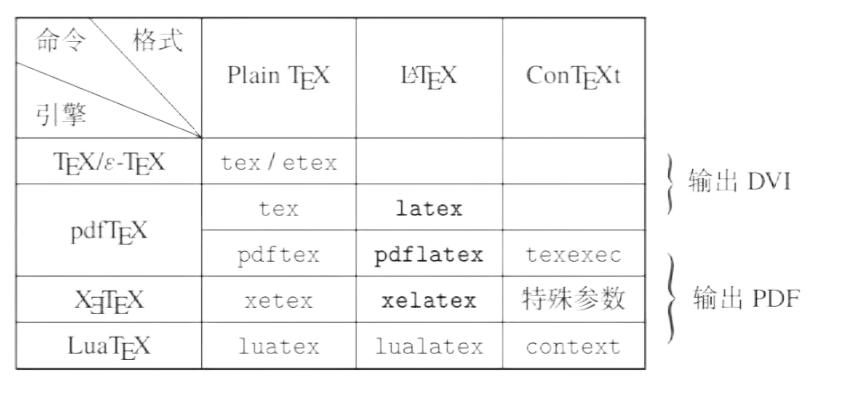
\includegraphics[width=0.5\textwidth]{tex引擎.jpg}
    \end{figure}

    \qquad 使用 \LaTeX 格式的排版得到 PDF 文件的方式也有好几种。其中使用 \lstinline{latex + dvips} 的方式最为古老,不便于中文文档的排版。用 \lstinline{latex} 和 \lstinline{pdflatex} 命令排版在处理中文时都使用 CJK 宏包的机制,而 \lstinline{xelatex} 则使用新的 xeCJK 宏包的机制。功能上 \lstinline{xelatex} 最为方便,尤其是在处理中文时;而用 \lstinline{pdflatex} 编译,一些宏包的兼容性会更好一些。不过本书的大部分内容并不限于任何一种模式,只是在处理中文时,将主要讨论 \lstinline{xelatex}。

    \begin{figure}[H]
        \centering
        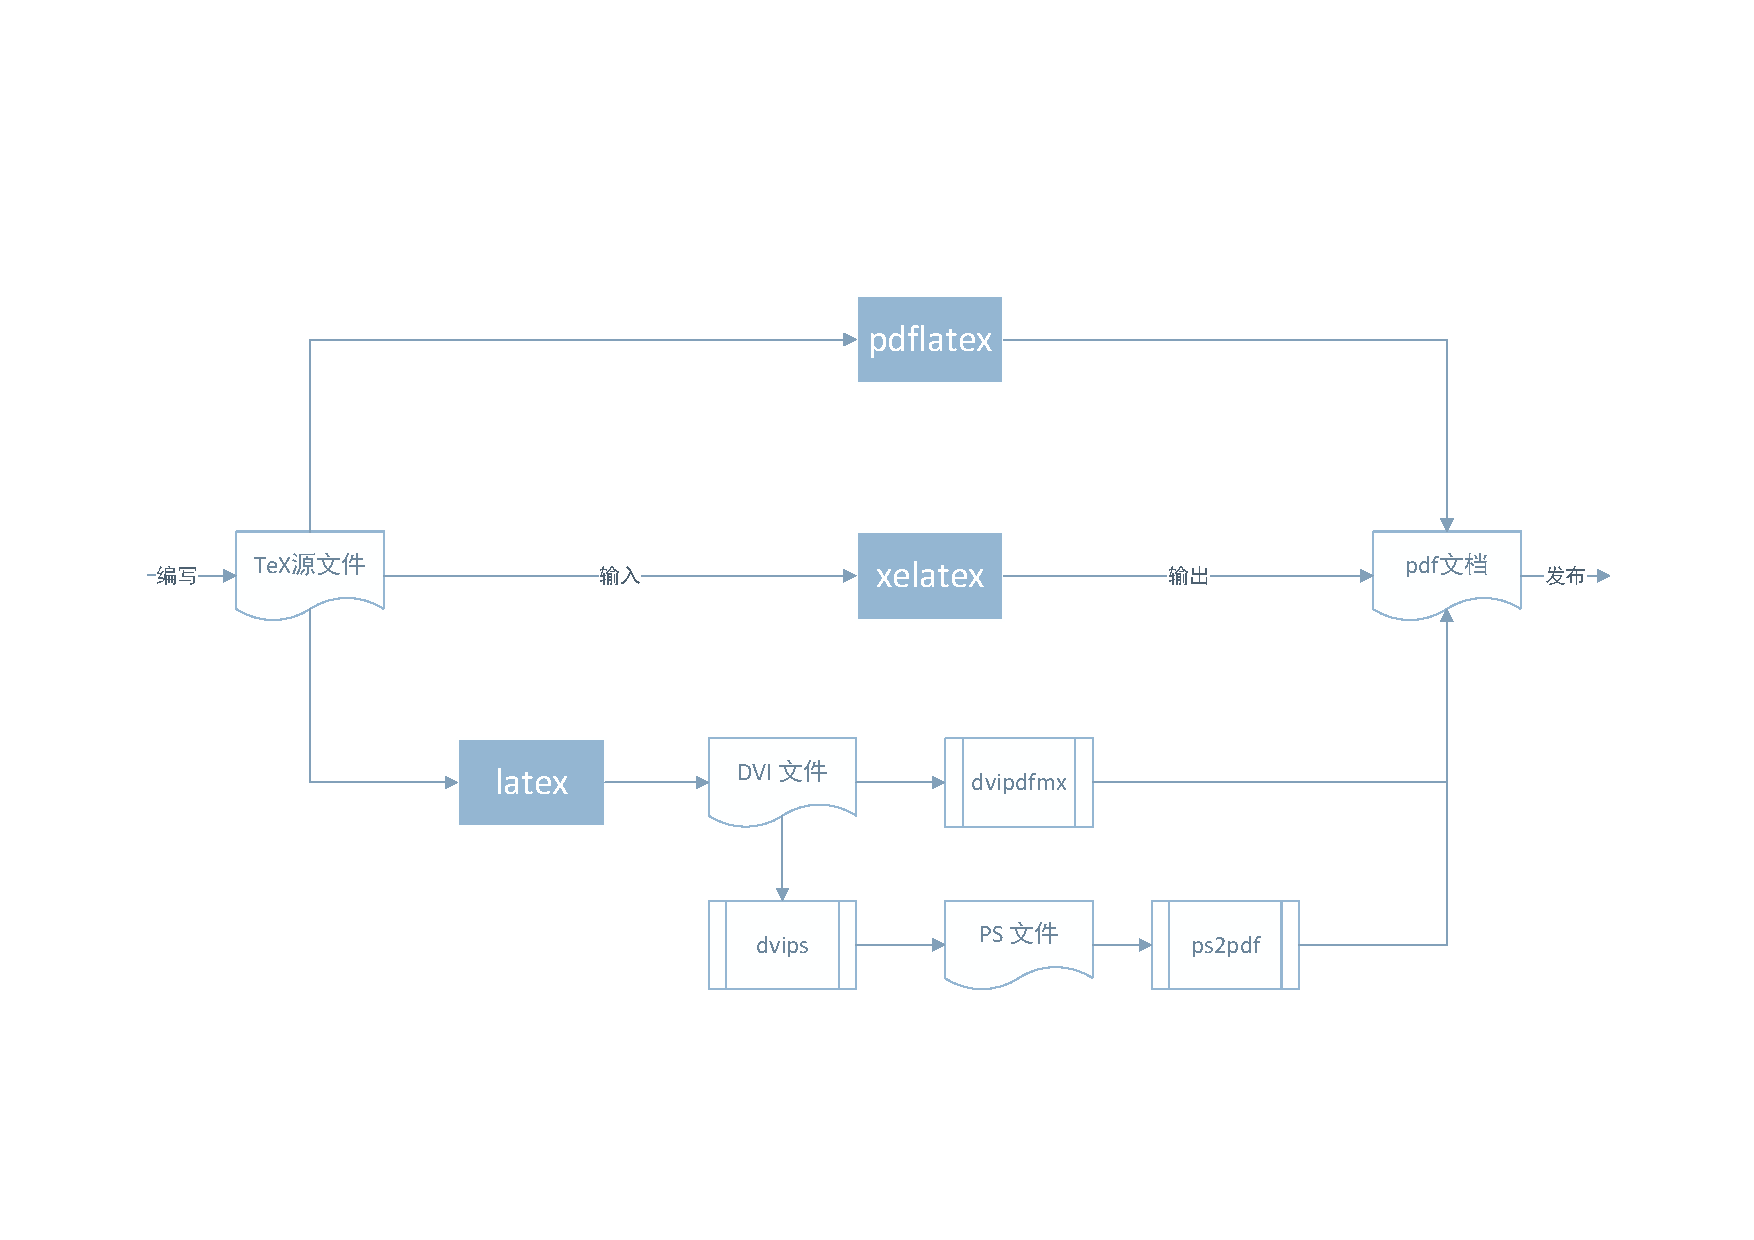
\includegraphics[width=0.5\textwidth]{编译成pdf.pdf }
    \end{figure}
}

\section{从一个例子说起}

这一节将研究一个相对实际的例子。在这个简单的例子中,我们将看到在真正的写作排版工作中常遇到的一些模式、问题的解决思路。有一些代码或许一时难以理解,不用担心,我们将在后面的章节里面详细讨论。

\subsection{确定目标}

现在来把话题限定在初等平面几何,假定我们要写一篇关于勾股定理的短文,短文是一般的科技论文的模式,结构上包括标题、摘要、目录、几节的正文和最后的参考文献;内容包括文字、公式、图形、表格等。短文的格式很平凡,没有什么特别的地方,但也足够实际,可以代表大多数使用\LaTeX 的人日常接触最多的文档类型,只不过现实中的例子在内容上比这里的例子更丰富、更深刻。

为了能在书中方便地显示这个例子,我们把短文的页面设置的很小,四页拼成一页,完成的样子如图\ref{fig:gougu}所示。如果你以前已经对 \LaTeX 有一些基础,不妨自己动手排一下这个小例子(不偷看本章后面的说明),看看你能否准确高效地完成;即使你对\LaTeX 的实际了解有限,也不妨考虑一下,在这个极其简单的例子中,有哪些内容需要表现,它们对应的形式是什么,需要注意哪些问题。

\begin{figure}
    \centering
    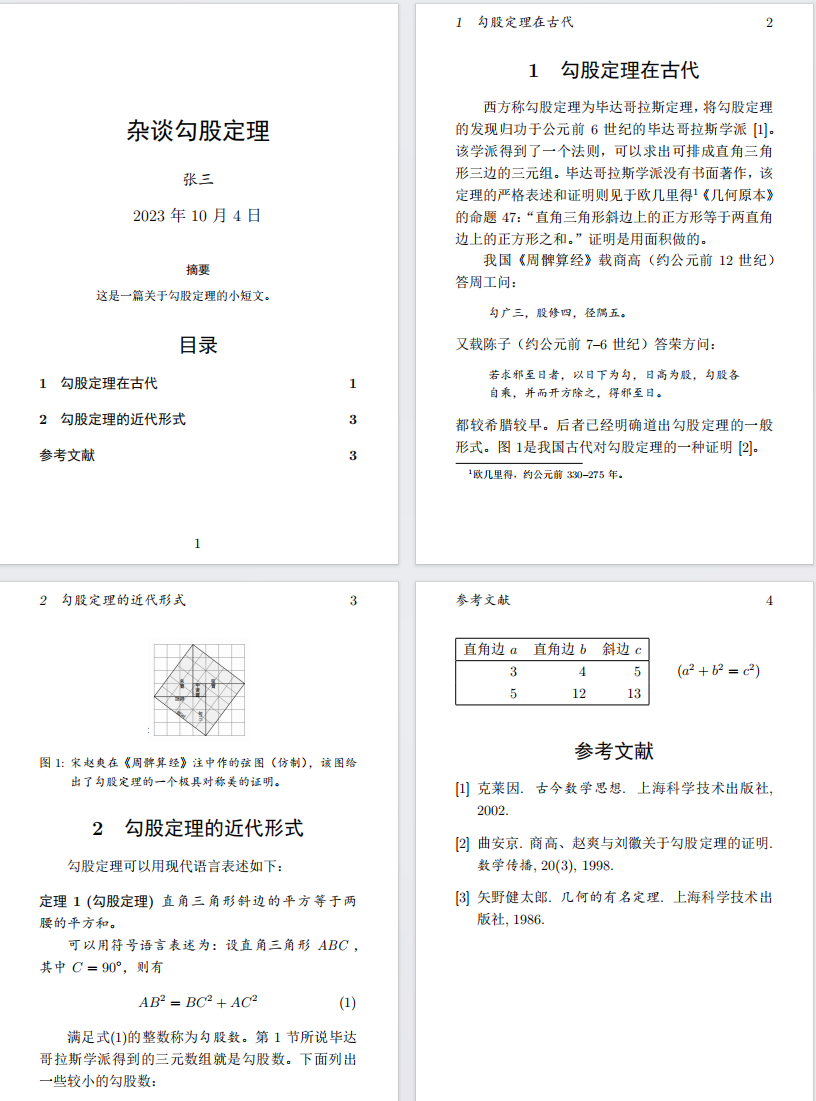
\includegraphics[width=\textwidth]{杂谈勾股定理.png}
    \caption{完整排版的小例子}
    \label{fig:gougu}
\end{figure}
\subsection{从提纲开始}

无论是对已经写好的文章进行排版,还是从零开始直接写文章,从提纲开始都是一个好主意。写出\LaTeX 文档的框架,进行必要的基本设置,然后再填入内容就方便了。

我们的例子《杂谈勾股定理》的提纲如下:

\begin{lstlisting}[numbers=left]
    % -*- coding: UTF-8 -*-
    % gougu.tex
    % 勾股定理
    \documentclass[UTF8]{ctexart}

    \title{杂谈勾股定理}
    \author{张三}
    \date{\today}

    \bibliographystyle{plain}

    \begin{document}

    \maketitle
    \tableofcontents
    \section{勾股定理在古代}
    \section{勾股定理的近代形式}
    \bibliography{math}

    \end{document}
\end{lstlisting}

源文件的一些东西我们已经见过了,也有一些是没见过的。但可以看出整个文章的框架,现逐条进行说明:

\begin{itemize}
    \item 前面以百分号\% 开头的是\textbf{注释}。在\TeX 中,源文件一行中\% 后的内容都会被忽略。这里有三行注释,第1行表明了这个文档的编码是 UTF-8 ,这对中文文档往往非常有用;第2行是源文件的文件名\verb|gougu.tex|;第三行则说明了源文件的内容。注释并不是\TeX 源文件必需的,这里对文件内容的注释似乎与文档标题重复,不过对于比较大的文档,源文件往往分成几个文件,这类说明性文字就十分重要了。
    \item 第4行是\textbf{文档类},因为是中文的短文,所以使用 ctexart ,并用\verb|[UTF8]|选项说明编码。
    \item 第6行至第8行,声明了整个文章的\textbf{标题}、\textbf{作者}和\textbf{写作日期},其中\verb|\today| 当然是“今天”的日期。这些信息并不马上出现在编译的结果中,而要通过第14行的\verb|\maketitle|排版。
    \item 第10行的\verb|\bibliographystyle|声明\textbf{参考文献}的格式。
\end{itemize}

以上在\verb|\begin{document}|之前的部分称为\textbf{导言区}( preamble ) ,导言区通常用来对文档的性质做一些设置,或者自定义一些命令。

\begin{itemize}
    \item 第12行和第20行以\verb|\begin{document}|和\verb|\end{document}| 声明了一个 \verb|document| 环境,里面是论文的正文部分,也就是直接输出的部分。
    \item 第14行的\verb|\maketitle|命令实际输出论文标题。
    \item 第15行的\verb|\tableofcontents|命令输出目录。
    \item 第16至17行的两个\verb|\section|开始新的一节。
    \item 最后第18行的\verb|\bibliography{math}| 则是提示\TeX 从文献数据库 \verb|math|中提取文献信息,打印参考文献列表。
\end{itemize}

为了格式上的清晰,源文件中适当加入了一些空行作为分隔。在正文外的部分,空行不代表任何意义。

这里的提纲非常简单,整个文档也没有什么复杂的层次结构。编译提纲将得到只有一些标题的文件。我们并没有写任何编号或数字,所有编号、包括目录和页码都是自动生成的。注意这里生成目录至少要编译两次,让\LaTeX 有机会读完整个论文来计算目录结构。

\subsection{填写正文}

\begin{lstlisting}[showspaces=true,numbers=left]
西方称勾股定理为毕达哥拉斯定理,将勾股定理的发现归功于公元前 6 世纪的毕达哥拉斯学派。该学派得到了一个法则,
可以求出可排成直角三角形三边的三元数组。毕达哥拉斯学派没有书面著作,该定理的严格表述和证明则见于欧几里得《
几何原本》的命题 47:“直角三角形斜边上的正方形等于两直角边上的正方形之和。”证明是用面积做的。

我国《周髀算经》载商高(约公元前 12 世纪)答周工问……
\end{lstlisting}

填写正文的部分看起来比较简单,就是直接填写大段的文字,不过仔细查看代码,也有如下一些要注意的地方(这里用\lstinline[showspaces=true]{ }表示空格。

\begin{itemize}
    \item \textbf{使用空行分段}。单个换行并不会使文字另起一段,而只是起到使源代码更易读的作用。空白行,也就是至多有空白的行,会使文字另起一段。空行只是起分段的作用,使用很多空行并不起增大段间距的作用。
    \item \textbf{段前不用打空格}。\LaTeX 会自动完成文字的缩进。即使手工在前面打了空格,\LaTeX 也会将其忽略,事实上它会忽略每行开始的所有空格。也不要使用全角的汉字空格,这通常会使排版的效果变得糟糕。
    \item \textbf{通常汉字后面的空格会被忽略,而其它符号后面的空格则会保留},因而用\lstinline[showspaces=true]{左 右}|就得到连续的“左右”,但\lstinline[showspaces=true]{left right}就会输出有空格的“ left right ”。单个的换行就相当于一个空格,因此源代码中大段文字可以安全地分成短行。空格只起分隔单词或符号的作用,使用很多空格并不起任何增大字词间距的作用。使用\verb|xelatex| 编译文档,ctexart 文档类会调用 xeCJK 宏包,自动处理汉字与其他符号之间的距离,无论你有没有在它们之间加上正确的空格,这是十分方便的。不过,在源代码中仍然可以给汉字与其它符号之间加上一个空格,这会使代码更加清晰。
\end{itemize}

换行与空格的使用,正是在\LaTeX 中文字排版中最基本的部分,却也是最容易被忽略的。现在你的心思可能早已经飘到脚注和《周髀算经》的引用这些显眼的地方了,但在进行下一步之前最好还是巩固一下前面的内容。

\subsection{命令与环境}

继续排版短文的第1节,我们来处理脚注和引用内容。

脚注是在正文“欧几里得”的后面用脚注命令\verb|\footnote|得到的:
\begin{lstlisting}
    ……见于欧几里得\footnote{欧几里得,约公元前330--275年。}《几何原本》的……
\end{lstlisting}
在这里,\verb|\footnote| 后面的花括号内的部分是命令的参数,也就是脚注的内容。

文中还使用\verb|\emph|命令改变字体形状,表示强调( emphasis )的内容:
\begin{lstlisting}
    ……满足式的整数称为\emph{勾股数}。……
\end{lstlisting}

一个\LaTeX 命令(宏)的格式为:
\begin{lstlisting}
    无参数:        \command
    有n个参数       \command{arg1}{arg2}……{argn}
    有可选参数      \command[opt args]{arg1}{arg2}……{argn}
\end{lstlisting}

命令都以\verb|\| 开头,后接命令名,命令名或者是一串字母,或是单个符号。命令可以带一些参数,如果命令的参数不止一个字符(不包括空格),就必须用花括号括起来。可选参数如果出现,则用方括号括起来。这里的脚注命令\verb|\footnote| 就是带有一个参数的命令,前面看到的\verb|\documentclass| 就是一个能带可选参数的命令。

引用的内容则是在正文中使用\verb|quote| 环境得到的。
\begin{lstlisting}
    ……答周工问:
    \begin{quote}
        勾广三,股修四,径隅五。
    \end{quote}
    又载陈子(约公元前 7--6 世纪答荣方问:
    \begin{quote}
        若求邪至日者,以日下为勾,日高为股,勾股各自乘,并而开方除之,得邪至日。
    \end{quote}
    都较希腊较早。……
\end{lstlisting}
\verb|quote|环境即以\verb|\begin{quote}| 和 \verb|\end{quote}| 为起止位置的部分。它将环境中的内容单单独分行,增加缩进和上下间距排版,以突出引用的部分。

不过,如果只使用\verb|quote| 环境,并不能达到预期的效果:\verb|\quote| 环境并不改变引用内容的字体,因此还需要再使用改变字体的命令,即:
\begin{lstlisting}
    \begin{quote}
        \zihao{-5} \kaishu
        勾广三,股修四,径隅五。
    \end{quote}
\end{lstlisting}
这里,\verb|\zihao| 是一个带有参数的命令,选择字号(-5 就是小五号);而 \verb|\kaishu| 则是一个没有参数的命令,把字体切换为楷书,注意用空格把命令和后面的文字分开。

类似地,文章的摘要也是在\verb|\maketitle| 之后用 \verb|abstract| 环境生成的:
\begin{lstlisting}
    \begin{abstract}
        这是一篇关于勾股定理的小短文。
    \end{abstract}
\end{lstlisting}

摘要环境的预设已经满足我们的要求了,不必再修改了。

上面使用的选择字体字号的命令与之前的脚注命令不同。\verb|\footnote{内容}| 只在原地发生效果,即生成脚注;但\verb|\zihao{字号}| 与 \verb|\kaishu| 命令则会影响后面的所有文字,直到整个分组结束。这种命令又称为声明( declaration )。

分组限定了声明的作用范围。一个 \LaTeX 环境天生就是一个分组( group ),因此前面的字号、字体命令会影响整个 \verb|quote| 环境。最大的分组是表示正文的 \verb|document| 环境,也可以用成对的花括号 \verb|{ }| 产生一个分组。

\LaTeX 环境( environment )的一般格式是:
\begin{lstlisting}
    \begin{环境名}
        环境内容
    \end{环境名}
\end{lstlisting}

有的环境也有参数或可选参数,格式为:
\begin{lstlisting}
    \begin{环境名}[可选参数]{其它参数}
        环境内容
    \end{环境名}
\end{lstlisting}

\verb|quote| 环境是无参数的,后面我们很快会在制作表格时遇到有参数的环境。

文章第二节的定理,是用一类定理环境输出的。定理环境是一类环境,在使用前需要在导言区做定义:
\begin{lstlisting}
    \newtheorem{thm}{定理}
\end{lstlisting}
这就定义了一个叫\verb|thm| 的环境。定理环境可以有一个可选参数,就是定理的名字。于是前面的勾股定理就可以由新定义的\verb|thm| 环境得到:
\begin{lstlisting}
    \begin{thm}[勾股定理]
        直角三角形斜边的平方等于两腰的平方和。
    
        可以用符号语言表述为……
    \end{thm}
\end{lstlisting}

最后来注意一个小细节,前面在表示起迄年份时,用了两个减号\verb|--| ,这在 \LaTeX 中将输入一个“ en dash ”,即宽度与字母“ n ”相当的短线,通常用来表示数字的范围。

\subsection{遭遇数学公式}

现在来看我们最关心的问题——输入数学公式,这大概是多数使用\LaTeX 的人花费精力最多的地方了。

最简单的输入公式的办法是把公式用一对美元符号\verb|$ $| 括起来,如使用\verb|$a+b$| 就得到漂亮的 $a+b$ ,而不是直接输入 \verb|a+b| 得到干巴巴的 a+b 。这种夹在行文之中的公式称为“正文公式”( in-text formula ) 或“行内公式” ( inline formula )。

对比较长或比较重要的公式,一般单独居中写在一行;为了方便引用,经常还给公式编号。这种公式称为“显示公式” 或 “列表公式”( displayed formula ),使用\verb|equation| 环境就可以方便地输入这种公式:

\begin{minipage}[t]{0.45\textwidth}
    \begin{lstlisting}
    \begin{equation}
        a(b+c) = ab + bc
    \end{equation}
    \end{lstlisting}
\end{minipage}
\hfill
\begin{minipage}[t]{0.45\textwidth}
    \begin{equation}
        a(b+c) = ab + bc
    \end{equation}
\end{minipage}

键盘上没有的符号,就需要一个命令来输入。例如表示“角”的符号$\angle$ 就可以用\verb|\angle| 来输入。命令的名字通常就是符号的名字,“角”的符号是\verb|\angle|,希腊字母$\pi$ 也就用其拉丁拼写\verb|\pi|。用命令表示的数学符号在\LaTeX 中使用起来与用键盘输入的数学符号用起来没有什么差别:

\begin{minipage}[t]{0.45\textwidth}
    \begin{lstlisting}
    $\angle ACB = \pi / 2$
    \end{lstlisting}
\end{minipage}
\hfill
\begin{minipage}[t]{0.45\textwidth}
    \vspace{0.1cm}
    \hspace{2.8cm} $\angle ACB = \pi / 2$
\end{minipage}

数学公式不只是符号的堆砌,还具有一定的数学结构,如上下标、分式、根式等。在勾股定理的表述中,就用到了上标结构表示乘方:

\begin{minipage}[t]{0.45\textwidth}
    \begin{lstlisting}
    \begin{equation}
        AB^2 = BC^2 + AC^2 
    \end{equation}
    \end{lstlisting}
\end{minipage}
\hfill
\begin{minipage}[t]{0.45\textwidth}
    \begin{equation}
        AB^2 = BC^2 + AC^2 
    \end{equation}
\end{minipage}

符号\verb|^| 用来引入一个上标,而\verb|_| 则引入一个下标,它们用起来差不多等同于一个带有一个参数的命令,因此多个字符的上下标需要用花括号分组,如\verb|$2^{10}=1024$| 得到 $2^{10}=1024$。

怎么输入$90^{\circ}$?如果去查数学符号表,你可能一无所获,由于\LaTeX 默认的数学字体中,并没有一个专门用于表示角度的符号,自然也就没有这个命令。角度的符号$^{\circ}$ 是通过上标输入的:\verb|$^{\circ}$|。这里的\verb|\circ| 其实是一个通常用来表示函数复合的二元运算符“$\circ$” ,我们把它的上标形式借用来表示角度,$90^{\circ}$ 可以用 \verb|$90^{\circ}$| 输入。

这篇小短文用到的数学公式暂且就只有这么多,我们将在第4章再来深入探讨这个话题。

\subsection{使用图表}

准备图表比起输入文字和公式就要麻烦一些了,很多人能够驾驭十分复杂的数学公式,却往往在图表问题上一筹莫展。这篇关于勾股定理的短文使用的图表形式都比较简单,但也是典型的。

首先来看插图。在 \LaTeX 中使用插图有两种途径,一是插入事先准备好的图片,二是使用 \LaTeX 代码直接在文档中画图。大部分情况下都是使用插入外部图片的形式,只有在一些特别的情况下才大量用代码作图(如数学的交换图)。

插图功能不是由 \LaTeX 的内核直接提供的,而是由 graphicx 宏包提供。要使用 graphicx 宏包 的插图功能,需要在源文件的导言区使用 \verb|\usepackage| 命令引入宏包:

\begin{lstlisting}
    \documentclass[UTF8]{ctexart}
    \usepackage{graphicx}
    % ……导言区其他内容
\end{lstlisting}

引入 graphicx 宏包之后,就可以使用\verb|\includegraphics| 命令插图了:

\begin{minipage}[t]{0.45\textwidth}
    \begin{lstlisting}
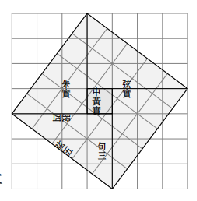
\includegraphics[width=3cm]{xiantu.pdf}
    \end{lstlisting}
\end{minipage}
\hfill
\begin{minipage}[m]{0.45\textwidth}
    \vspace{0.1cm}
    \hspace{2.5cm} 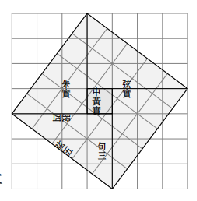
\includegraphics[width=3cm]{xiantu.pdf}
\end{minipage}

这里\verb|\includegraphics| 有两个参数,方括号中的可选参数\verb|width=3cm| 设置图形在文档中显示的宽度为 3 cm ,而第二个参数 \verb|xiantu.pdf| 则是图形的文件名(放在源文件目录)。有最常见的情况,图形使用其他画图工具做好,但在制作的时候尺寸不符合文章的要求,需要在插图时设置参数缩放到指定的大小。还有一些类似的参数,如\verb|scale=缩放因子|、\verb|height=高度| 等,我们在这篇小短文中实际使用的是\verb|scale=0.8|。插图命令支持的图形文件格式与所使用的编译程序有关,这篇中文文章使用 xelatex 命令编译,支持的图形格式包括 PDF、PNG、JPG、EPS 等,这里的图形实际是利用 Asymptote 语言制作的。

插入的图形就是一个有内容的矩形盒子,在正文中和一个很大的字符没有区别。因此如果把插图和文字混在一起,就会出现这样的情况:

\begin{minipage}[t]{0.45\textwidth}
    \begin{lstlisting}
    文字文字
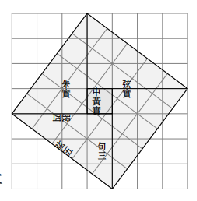
\includegraphics[width=3cm]{xiantu.pdf}
    text text
    \end{lstlisting}
\end{minipage}
\hfill
\begin{minipage}[c]{0.45\textwidth}
    \vspace{0.1cm}
    \hspace{2.5cm}
    文字文字
    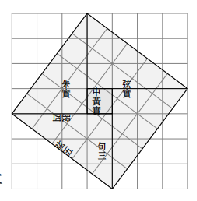
\includegraphics[width=3cm]{xiantu.pdf}
    text text
\end{minipage}

除了一些很小的图标,我们很少把插图直接夹在文字之间,而是使用单独的环境列出。而且很大的图形如果固定位置,会给分页造成困难。因此,通常都把图形放在一个可以变动相对位置的环境中,称为“浮动体”( float )。在浮动体中还可以给图形加入说明性的标题,因此,在《杂谈勾股定理》中实际是使用下面的代码插图的:
\begin{lstlisting}[numbers=left]
    \begin{figure}[ht]
        \centering
        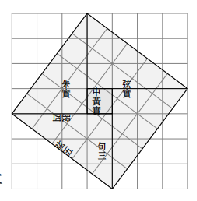
\includegraphics[scale=0.6]{xiantu.pdf}
        \caption{宋赵爽在《周髀算经》注中作的弦图(仿制),该图给出了勾股定理的一个极具对称美的证明。}
        \label{fig:xiantu}
    \end{figure}
\end{lstlisting}

在上面的代码中,第 1 行和第 6 行使用了\verb|figure| 环境,就是插图使用的浮动体环境。\verb|figure| 环境有可选参数\verb|ht|,表示浮动体可以出现在环境周围的文本所在处( here ) 和一页的顶部( top ) 。 \verb|figure| 环境内部相当于普通的段落(默认没有缩进);第 2 行用声明\verb|\centering| 表示后面的内容居中;第 3 行插入图形;第 4 行和第 5 行使用\verb|\caption| 命令给插图加上自动编号和标题;第 6 行的\verb|\label| 命令则给图形定义一个标签,使用这个标签就可以在文章的其他地方引用\verb|\caption| 产生的编号(编号引用我们会在后面讲到)。这段插图的代码非常格式化,在绝大多数情况下,文章中的插图都是用与这里几乎完全一样的代码插入的。

下面再来看表格。插图可以用其他软件做好插入,但表格一般都是在 \LaTeX 里面完成的。制作表格,需要确定的是表格的行、列对齐模式和表格线,这是由\verb|tabular| 环境完成的:

\begin{minipage}[t]{0.45\textwidth}
    \begin{lstlisting}
        \begin{tabular}{|rrr|}
            \hline
            直角边 $a$ & 直角边 $b$ & 斜边 $c$ \\ 
            \hline
            3 & 4 & 5 \\ 
            5 & 12 & 13 \\ 
            \hline
        \end{tabular}
    \end{lstlisting}
\end{minipage}
\hfill
\begin{minipage}[t]{0.45\textwidth}
    \vspace{0.1cm}
    \hspace{0.5cm}
    \begin{tabular}{|rrr|}
        \hline
        直角边 $a$ & 直角边 $b$ & 斜边 $c$ \\ 
        \hline
        3 & 4 & 5 \\ 
        5 & 12 & 13 \\ 
        \hline
    \end{tabular}
\end{minipage}

\verb|tabular| 环境有一个参数,里面声明了表格中列的模式。在前面的表格中,\verb||rrr|| 表示表格有三列,都是右对齐,在第一列前面和第三列后面各有一条垂直的表格线。在\verb|tabular| 环境内部,行与行之间用命令\verb|\\| 隔开,每行内部的表项用符号\verb|&| 隔开。表格中的横线则是用命令 \verb|\hline| 产生的。

表格与\verb|\includegraphics| 命令得到的插图一样,都是一个比较大的盒子。一般也放在浮动环境中,即\verb|table| 环境,参数与大体的使用格式也与\verb|figure| 环境差不多,只是\verb|\caption| 命令得到的标题是“表”而不是“图”。在《杂谈勾股定理》中,我们稍稍改变了一下\verb|figure| 环境通常的内容:

\begin{minipage}[t]{0.45\textwidth}
    \begin{lstlisting}
        \begin{table}[H]
            \begin{tabular}{|rrr|}
                \hline
                直角边 $a$ & 直角边 $b$ & 斜边 $c$ \\ 
                \hline
                3 & 4 & 5 \\ 
                5 & 12 & 13 \\ 
                \hline
            \end{tabular}%
            \qquad
            ($a^2 + b^2 = c^2$)
        \end{table}
    \end{lstlisting}
\end{minipage}
\hfill
\begin{minipage}[t]{0.45\textwidth}
    \vspace{0.1cm}
    \hspace{0.5cm}
    \begin{table}[H]
        \begin{tabular}{|rrr|}
            \hline
            直角边 $a$ & 直角边 $b$ & 斜边 $c$ \\ 
            \hline
            3 & 4 & 5 \\ 
            5 & 12 & 13 \\ 
            \hline
        \end{tabular}%
        \qquad
        ($a^2 + b^2 = c^2$)
    \end{table}
\end{minipage}

这里并没有给表格加标题,也没有把内容居中,而是把表格与一个公式并排排开,中间使用一个 \verb|\qquad| 分隔。命令 \verb|\qquad| 产生长为 2em (大约两个“ M ”的宽度)的空白。因为我们已经使用\verb|\qquad| 生成足够长度的空格了,所以再用\verb|\end{tabular}| 后面的注释符取消换行产生的一个多余的空格,这正好达到我们的预期效果。

之所以使用这种方式防止表格,是因为在正文中表格前面写道:

{\qquad \heiti \zihao{-5} …… 下表列出一些较小的勾股数:}

也就是说表格和正文是直接连在一起的,而且后面的公式也说明了表格的意义,自然也就不需要多余的标题了,这样一来表格就于正文连在一起,不允许再浮动了,因而这里本来是不应该使用浮动的\verb|table| 环境的,但我们仍然使用了\verb|table| 环境,在表示位置的参数处使用了\verb|[H]| ,表示“就放在这里,不浮动”。\verb|[H]| 选项并不是标准 \LaTeX 的\verb|table| 的参数,而是由 float 宏包提供的特殊功能。因此要让上面的代码正确运行,还要在导言区使用\verb|\usepackage{float}| 。在这种表格很小(不影响分页) ,行文又要求连贯的场合, float 宏包的这种不浮动的图表环境是很有用的。

\subsection{自动化工具}

到目前为止,《杂谈勾股定理》这篇小文的大部分内容已经排完了,如果把前面提到的所有代码结合在一起,装进一个文件,差不多就能得到一篇完整的文章了——这里说“差不多”,其实还缺少一些重要的东西,最明显的就是参考文献列表。

你一定已经注意到了,在前面文档的提纲中,我们已经用\verb|\bibliographystyle| 命令声明了参考文献的格式,又用\verb|\bibliography| 命令要求打印出参考文献列表。不过,这只是使用 BibTeX 处理文献的一个空架子,我们尚没有定义“参考文献数据库”,自然也不会产生任何文献列表。

BibTeX 使用的参考文献数据库其实就是一个后缀为\verb|.bib| 的文件。我们的《杂谈勾股定理》使用了一个包含 3 条文献的数据库文件 \verb|math.bib| ,内容如下:
\begin{lstlisting}
    % This file was created with JabRef 2.6
    % Encoding: UTF8

    @BOOK{Kline,
        title = {古今数学思想},
        publisher = {上海科学技术出版社},
        year = {2002},
        author = {克莱因}
    }

    @ARTICLE{quanjing,
        author = {曲安京},
        title = {商高、赵爽与刘徽关于勾股定理的证明},
        journal = {数学传播},
        year = {1998},
        volume = {20},
        number = {3}
    }

    @BOOK{Shiye,
        title = {几何的有名定理},
        publisher = {上海科学技术出版社},
        year = {1986},
        author = {矢野健太郎}
    }
\end{lstlisting}

正如上面所看到的,一个文献数据库文件的格式并不复杂,每则文献包括类型、引用标签、标题、作者、出版年、出版社等信息,可以直接手工输入。不过正像前面数据库文件的注释(以\% 开头的两行)所显示的那样,这个数据库文件并不是直接输入上面的文件内容得到的,而是使用文献管理工具 JabRef 制作的。

在现实中, BibTeX 数据库经常并不需要我们自己录入,而可以从相关学科的网站直接下载或是从其他类型的文献数据库转换得到。即使是在需要我们自己录入的情况下,使用 JabRef 这种软件来管理也更方便,不易出错。

BibTeX 是一个专门用于处理 \LaTeX 文档文献列表的程序吗,使用 BibTeX 处理文献时,编译 \verb|gougu.tex| 这一个文档的步骤就增加为四次运行程序(或点击四次按钮):
\begin{lstlisting}
    xelatex gougu.tex  
    bibtex gougu.tex  
    xelatex gougu.tex  
    xelatex gougu.tex
\end{lstlisting}
第一次运行 \verb|xelatex| 为 BibTeX 准备好辅助文件,确定数据库中的哪些文献将被列出来。然后\verb|\bibtex| 处理辅助文件 \verb|gougu.tex| ,从文献数据库中选取文献,按照指定的格式生成文献列表的 \LaTeX 代码。后面两次 \verb|xelatex| 再读入文献列表代码并生成正确的引用信息。这种利用多躺编译处理辅助文件的方式看起来有些复杂,但这是使用自动文献生成的代价之一,不过好处也是明显的,文献的管理、文献列表的排序和排版格式等都能高效漂亮地完成。

如果现在就使用上面的步骤编译,你仍然会一无所获,因为还没有选择要列出的文献。\LaTeX 只选择被引用的文献。引用文献的方法是在正文中使用\verb|\cite| 命令,如:

\begin{lstlisting}
    西方称勾股定理为毕达哥拉斯定理,将勾股定理的发现归功于公元前 6 世纪的毕达哥拉斯学派\cite{Kline}。

    ……是我国古代对勾股定理的一种证明\cite{quanjing}。
\end{lstlisting}
\verb|\cite| 命令的参数 Kline 和 quanjing 分别是其中两篇文献的引用标签,也就是在 \verb|math.bib| 中每个条目第一行出现的东西。使用 \verb|\cite| 命令会在引用的位置显示文献在列表中的编号(它在第 3 次 \verb|xelatex| 编译之后才能确定),同时在辅助文件中说明某文献将被引用。如果要在列表中显示并不直接引用的文献,可以使用 \verb|\nocite| 命令,一般是把它放在\verb|\bibliography| 之前,像我们这篇文章一样:

\begin{lstlisting}
    \nocite{Shiye}
    \bibliography{math}
\end{lstlisting}

有了上面的引用代码,加上完整的数据库文件,通过多步编译,最终就能得到文献列表。

BibTeX 是这篇文章用到的最复杂的自动化工具,最简单的自动化工具则是页码、定理和公式的自动编号,其余的还包括生成目录与图表公式的交叉引用。

目录也是自动从章节命令中提取并写入目录文件的,我们在提纲中就使用了\verb|\tableofcontents| 命令,它将在第二次 \verb|xelatex| 编译时生效。

引用不仅限于参考文献。图表、公式的编号,只要事先设定了标签,同样可以通过辅助文件为中介引用。基本的交叉引用命令是\verb|\ref| ,它以标签为参数,得到被引用的编号。例如,在插图时已经用\verb|\label| 命令为弦图定义了标签\verb|fig:xiantu|,于是,在正文中就可以使用
\begin{lstlisting}
    图\ref{fig:xiantu} 是我国古代对勾股定理的一种证明 \cite{quanjing}。
\end{lstlisting}
来对弦图的编号进行引用。

公式编号的应用也可照此办理,不过需要在公式中定义标签:
\begin{lstlisting}
    \begin{equation}\label{eq:gougu}
        AB^2 = BC^2 + AC^2 
    \end{equation}
\end{lstlisting}
而后在正文中以\verb|\ref{eq:gougu}| 引用。实际中引用公式非常常用,数学宏包 amsmath 就定义了 \verb|\eqref| 命令,专门用于公式的引用,并能产生括号:
\begin{lstlisting}
    % 导言区使用 \usepackage{amsmath}
    满足式 \eqref{eq:gougu} 的整数称为 \emph{勾股数}。
\end{lstlisting}

\subsection{设计文章的格式}

写到这里,原先的提纲骨架已经变成一篇完整的文章,似乎已经没有什么可说的了。然而,\TeX 的精神是精益求精、追求完美,如果我们对比预定的目标来审视我们现在排版的结果,还是会发现有些不同,如标题的字体还需要修正,目录中少了“参考文献” 一项,插图标题的字体、字号和对齐都不正确等。更重要的还有,目标预设的文章页面很小,页边距也非常紧凑,与现在宽大的页面大相径庭。这些都属于文章的整体格式,需要进一步的设计完善。

绝大部分设计工作是在文章的导言区通过一些命令定义和参数设定来完成的,但往往相当复杂,好在其中的大多数工作可以通过使用一些宏包来简化,前面已经用到过 graphicx 、 float 、 amsmath 几种宏包完成一些工作,这里也要用到几种。

设计页面尺寸可以使用 geometry 宏包:
\begin{lstlisting}
    \usepackage{geometry}
    \geometry{a6paper,centering,scale=0.8}
\end{lstlisting}
这是最简单的设定方式,定义页面使用 A6 纸大小,版心居中,长宽占页面的 0.8 倍。

改变图表标题格式可以使用 caption 宏包:
\begin{lstlisting}
    \usepackage[format=hang, font=small, textfont=it]{caption}
\end{lstlisting}
设定图表所有标题使用悬挂对齐方式(即编号向左突出),整体用小字号,而标题文本使用斜体(对汉字来说就是楷书)。

增加目录的项目则可以用 tocbibind 宏包:
\begin{lstlisting}
    \usepackage[nottoc]{tocbibind}
\end{lstlisting}
宏包默认会在目录中加入目录项本身、参考文献、索引等项目。这里使用 \verb|nottoc| 选项取消了在目录中显示目录本身。

标题和作者的字体可以直接在\verb|\title|、\verb|\author| 命令中设定,因为标题本身就是用这些命令在导言区定义的:
\begin{lstlisting}
    \title{\heiti 杂谈勾股定理}
    \author{\kaishu 张三}
    \date{\today}
\end{lstlisting}
其中\verb|\heiti| 是和 \verb|\kaishu| 类似的中文字体命令,把字体切换成黑体。

这篇短文到这里就全部排完了,不过正文中表示引用的\verb|quote| 环境里面还夹杂着字体命令,这种散落在各处的格式设置很难看清,而且不方便修改。为了解决这个问题,可以利用 \verb|\newenvironment| 命令定义一个新的环境,在原来\verb|quote| 的基础上再增加格式控制:
\begin{lstlisting}
    \newenvironment{myquote}
    { \begin{quote} \kaishu \zihao{-5} }
    { \end{quote} }
\end{lstlisting}
这里,\verb|\newenvironment| 有三个参数,第一个参数是环境的名字,后两个参数分别是在环境开始和末尾处的代码,因此,就可以使用新环境
\begin{lstlisting}
    \begin{myquote}
        勾广三,股修四,径隅五。
    \end{myquote}
\end{lstlisting}
来替换原来的\verb|quote| 环境了。如果此时需要修改引用的格式,那么只需要在导言区修改 \verb|myquote| 的定义,而不必在全文中搜索所有的\verb|quote| 环境的使用了。

类似地,原来数学公式中角度的单位\verb|^\circ| 也不直观,可以用 \verb|\newcommand| 命令定义一个新的命令\verb|\degree|:
\begin{lstlisting}
    \newcommand{\degree}{^\circ}
\end{lstlisting}
其中,\verb|\newcommand| 命令的两个参数分别是新命令和新命令的定义,于是我们就可以用 \verb|$90\degree$| 来代替原来不直观的$90^\circ$ 了。

在整篇文章编排结束之际,我们还是使用自定义的环境\verb|myquote| 和自定义的命令\verb|\degree| 代替了文中出现的特殊格式控制。类似地,在设定插图标题的字体时,并没有把字体、字号的命令塞进\verb|\caption| 命令的参数中,而是使用 \verb|\caption| 宏包统一管理。这样看起来比最“直接”的做法要多绕一道弯子,但好处是更清晰和更容易修改格式。这篇短文排在普通 A4 大小的纸张上只有一两页,还看不出什么特别之处,但当你开始编写和维护几十上百页的长文档时,在设计阶段所付出的精力就会得到回报了。

\LaTeX 是一种结构化的排版语言,在填写标准格式的模板时(就像我们前面写的提纲)可以忽略编号、格式等许多具体细节。在文档排版中应该主动追求内容与格式的分离,在\verb|document| 环境之内避免直接使用诸如字体字号、对齐缩进的格式控制命令,而取而代之的应该是有具体意义的环境和命令,让文档变得清晰。这种模式化的操作能够提高工作效率,许多 \LaTeX 的拥护者把这种工作方式称为“所想即所得”。可是不要忘记,机器还远没有智能化到想人之所想的程度,\LaTeX 也不能阻止我们编排出效果糟糕、代码混乱的文章,要想得到好的文章,无论是在内容上还是在排版形式上,都得靠我们自己。
